\documentclass[11pt, a4paper, parskip]{scrartcl}

\usepackage[margin=2.7cm]{geometry}
\usepackage{graphicx}
\usepackage{amsmath,paralist,xcolor,xspace,amssymb}
\usepackage{comment}
\usepackage[super]{nth}
\usepackage{seqsplit}
\usepackage{tikz}
\usepackage{multirow}
\usepackage{booktabs}
\usepackage{array}
\usetikzlibrary{positioning}
\usepackage[hidelinks]{hyperref}

\usepackage[]{natbib}
\bibliographystyle{apalike}

% Dev-doc, not a journal article: single column (via scrartcl above).
% \code{} is \texttt{} that may break mid-identifier/mid-path across
% lines (long function names, file paths) instead of overflowing the
% margin: used for long \texttt content in running text. Left as
% plain \texttt{} inside captions/section titles, where \seqsplit's
% \futurelet-based scanning cannot survive LaTeX's full expansion of
% moving arguments.
\newcommand{\code}[1]{\texttt{\seqsplit{#1}}}

% KOMA-Script disables the classic \rm/\bf/\it/... font-switch commands
% by default; the numbered sections use them freely for math-mode units
% (${\rm K}$, ${\rm cm^{-3}}$, ...), matching the old mnras.cls setup, so
% restore the standard LaTeX2e old-font-command behaviour here rather
% than editing every occurrence.
\makeatletter
\DeclareOldFontCommand{\rm}{\normalfont\rmfamily}{\mathrm}
\DeclareOldFontCommand{\sf}{\normalfont\sffamily}{\mathsf}
\DeclareOldFontCommand{\tt}{\normalfont\ttfamily}{\mathtt}
\DeclareOldFontCommand{\bf}{\normalfont\bfseries}{\mathbf}
\DeclareOldFontCommand{\it}{\normalfont\itshape}{\mathit}
\DeclareOldFontCommand{\sl}{\normalfont\slshape}{\@nomath\sl}
\DeclareOldFontCommand{\sc}{\normalfont\scshape}{\@nomath\sc}
\makeatother

\setkomafont{title}{\rmfamily\bfseries\boldmath}
\addtokomafont{section}{\rmfamily\bfseries\boldmath}
\addtokomafont{subsection}{\rmfamily\bfseries\boldmath}
\addtokomafont{subsubsection}{\rmfamily\bfseries\boldmath}

\newcommand{\todo}[1]{{\textcolor{red}{TODO: #1}\\}}
\newcommand{\swift}{{\sc Swift}\xspace}
\newcommand{\D}[2]{\frac{d#1}{d#2}}
\newcommand{\LL}{\left(}
\newcommand{\RR}{\right)}

\title{GEAR radiation feedback: radiation pressure and the FUV/ISRF}
\subtitle{Theory document: momentum injection, and the transport of the
far-ultraviolet light for photoelectric heating and H$_2$ photodissociation}
\author{Darwin Roduit}

\begin{document}
\maketitle

This is the \textbf{theory document} for two radiation feedback channels
beyond the subgrid HII photoionization model. The HII model has its own theory
document in this directory (\code{radiation.tex}). The two channels here are
largely self-contained:
\begin{itemize}
  \item the \textbf{radiation-pressure} channel, which injects momentum
    (Section~\ref{sec:radiation-pressure});
  \item the \textbf{FUV/ISRF} channel, which transports the far-ultraviolet
    light of the stars for photoelectric heating and H$_2$
    photodissociation (Section~\ref{sec:packet}).
\end{itemize}
The document describes the current design and physics only. Validation
results and open items live in the \textbf{GEAR radiation logbook}
(\code{swift-gear} repository, \code{theory/radiation/}). The HII theory
document and the logbook compile separately, so they are cited by name and
section, not by automatic cross-reference. Edit the numbered \code{.tex}
files directly; each covers one topic.

\textbf{In the code.} The radiation-pressure channel lives in
\code{src/feedback/GEAR/radiation.c} and related files, and the FUV/ISRF
channel in \code{src/feedback/GEAR/radiation\_isrf.c} and related files.

\tableofcontents

\section{Radiation pressure}
\label{sec:radiation-pressure}

This section documents the radiation-pressure feedback channel
(\code{GEARFeedback:radiation\_pressure\_efficiency}), a separate mechanism
from the HII photoionization budget documented in the algorithm
section of the HII photoionization theory document
(\code{radiation.tex}/\code{radiation.pdf}, this same directory):
photoionization tags and re-floors gas
temperature, while radiation pressure injects momentum directly into
gas neighbouring the star. The two channels draw on \emph{different}
integrals of the star's spectrum ($Q_H$ vs.\ $L_{\rm bol}$, see
Section~\ref{sec:rp-vs-hii} below) and use the same SPH gather around
the star, but are otherwise independent: a star can have one policy
enabled without the other. Not yet covered anywhere else in this
document; written up here for the first time.

\paragraph{Implementation.} The channel is the policy bit
\code{radiation\_policy\_radiation\_pressure}
(\code{src/feedback/GEAR\_thermal/feedback\_properties.h:58}), set at
\code{feedback\_properties.h:774} and tested in the apply loop at
\code{src/feedback/GEAR/radiation\_iact.h:252}.

\subsection{Physical distinction from photoionization}
\label{sec:rp-vs-hii}

Two genuinely different physical mechanisms in a real star, not two
bookkeeping categories of the same effect.

\textbf{Photoionization} is a quantum/atomic process: a photon with
energy above $13.6\,$eV (Lyman continuum, $\lambda<912\,$\AA) is
absorbed by a bound electron in hydrogen, ejecting it; the photon's
energy above the ionization threshold becomes the photoelectron's
kinetic energy, which thermalizes via collisions; this is what heats
the gas to $\sim10^4\,$K, balanced against recombination/line cooling.
Only photons above that specific energy threshold count, and the
relevant budget is $Q_H$ (ionizing photon \emph{number} rate, read from the pychem tables;
the blackbody-fit section of the HII photoionization theory document
describes how an entry can be understood), not energy.
This is fundamentally a \textbf{thermal/chemical} effect: it sets the
gas's ionization state and temperature, and in this code drives
dynamics only indirectly, through the resulting thermal-pressure
contrast against the cold ambient medium (the classical Spitzer D-type
expansion that STARBENCH, validated in the HII photoionization
logbook's own validation section, checks).

\textbf{Radiation pressure} is a mechanical process: \emph{any}
absorbed or scattered photon, at any wavelength, transfers momentum
$p=E/c$ to whatever absorbs or scatters it. This draws on $L_{\rm
bol}$: the star's entire spectrum, dominated for most stars by the
non-ionizing UV/optical continuum, not the ionizing band specifically
($L_{\rm bol}$ and $Q_H$ are separate entries of the pychem tables;
the HII photoionization theory document's blackbody-fit section
describes how such entries can be understood, not what SWIFT evaluates). It is
a \textbf{dynamical} effect: a direct push, independent of whether
the interaction happens to ionize anything, and in this code it acts
through Eq.~\ref{eq:rp-momentum-rate} directly, with no thermal
intermediary.

Two consequences worth keeping precise:
\begin{itemize}
  \item \textbf{They are not disjoint at the photon level.} An
    ionizing-photon absorption \emph{also} transfers momentum
    $h\nu/c$ in that same event: momentum conservation does not care
    about the atomic-physics outcome. But that ionizing-photon
    momentum is a small slice of the total budget, since $Q_H$
    photons are only part of $L_{\rm bol}$ for most stars, and dust
    reprocessing/IR trapping (the $(1+\tau_{\rm IR})$ term,
    Eq.~\ref{eq:rp-tauIR}) adds momentum from photons that were never
    ionizing to begin with. This code does not attempt to avoid
    double-counting this overlap; see the open interaction question
    in the GEAR radiation logbook's radiation-pressure open-questions
    section.
  \item \textbf{They drive HII region expansion through different,
    competing channels.} Photoionization heats gas against a cold
    ambient medium ($\sim10$--$100\,$K): the resulting
    \emph{thermal-pressure} contrast drives the D-type expansion.
    Radiation pressure drives expansion through \emph{direct momentum}
    deposition instead, no heating required.
    \citet{KrumholzMatzner2009}, already cited above for the Tier-2
    validation proposal, is literally a paper about comparing these
    two channels: thermal-pressure-driven expansion dominates for the
    modest OB associations STARBENCH-style tests represent, while
    radiation pressure only becomes the dominant \emph{dynamical}
    driver for far more luminous, compact sources (starburst clusters,
    super star clusters) where $L$ is large and the region is
    dense/compact enough for $\tau_{\rm IR}$ to matter.
\end{itemize}

\subsection{Momentum injection: single-scattering plus IR trapping}
\label{sec:rp-momentum}

Each active star's momentum injection rate is
\begin{equation}
  \dot p_{\rm rad} = \frac{L_{\rm bol}}{c}\,(1-e^{-\tau_{\rm NUV}})\,(1+\tau_{\rm IR}),
  \label{eq:rp-momentum-rate}
\end{equation}
implemented: the
$(1-e^{-\tau_{\rm NUV}})$ factor is the fraction of the star's non-ionizing
continuum actually absorbed before dust reprocessing, using
$\kappa_{\rm NUV}=1800\,{\rm cm^2\,g^{-1}}\,(Z/Z_\odot)$ (the value where
\citet{Hopkins2012a}'s single flux-mean estimate and
\citet{Hopkins2020}'s own NUV sub-band agree). The
standard single-UV-scattering-plus-dust-IR-trapping recipe: direct
absorption/scattering of the star's own UV/optical photons deposits
$L_{\rm bol}/c$ of momentum per unit time; photons re-radiated in the
IR by dust can scatter multiple times in an optically thick shell
before escaping, boosting the momentum transfer by a further factor of
$(1+\tau_{\rm IR})$ over a single scattering.

\textbf{Citation confirmed, direct primary-source check.}
This codebase's implementation is confirmed to be transcribed from
\citet{Hopkins2020} (the FIRE-2 radiative-feedback methods paper,
arXiv:1811.12462, distinct from the FIRE-2 numerics paper
\citet{Hopkins2018} already cited elsewhere in this document). Fetched
and grepped the full text directly: \citet{Hopkins2020}'s Appendix~A
gives \textbf{exactly}
$(\kappa_{\rm FUV},\kappa_{\rm NUV},\kappa_{\rm opt},\kappa_{\rm IR}) =
(2000, 1800, 180, 10)\,(Z/Z_\odot)\,{\rm cm^2\,g^{-1}}$: this
codebase's $\kappa_{\rm IR}=10\,{\rm cm^2\,g^{-1}}\,(Z/Z_\odot)$
(Eq.~\ref{eq:rp-tauIR}) matches precisely, not just order-of-magnitude.
\citet{Agertz2013}/\citet{Marinacci2019} remain plausible independent
lineages sharing the same functional form but are no longer the
open question: \citet{Hopkins2020} is confirmed as the actual source.

\textbf{The momentum-coupling factor.} \citet{Hopkins2020} \S4.4, footnote 16 (also
\citealt{Hopkins2014}, Appendix~A) gives the full LEBRON momentum-coupling
formula as $\dot p = \tilde\tau\,L_{\rm bol}/c$, with
$\tilde\tau = (1-e^{-\tau_{\rm single}})\,(1+\tau_{\rm eff,IR})$,
\emph{not} simply $(1+\tau_{\rm IR})$ as it would be without the first factor.
The $(1-e^{-\tau_{\rm single}})$ factor is the fraction of the
\emph{input} (non-ionizing UV/optical) luminosity actually absorbed before
reaching the dust that reprocesses it into the trapped IR term: the bare
$(1+\tau_{\rm IR})$ form implicitly assumes $\tau_{\rm single}\to\infty$ (full absorption),
which only holds deep in a dense cloud, over-estimating direct/single-
scattering radiation pressure at the production resolution this codebase
targets (10\,$M_\odot$ to a few $10^4\,M_\odot$ per gas particle), where
much of the coupling volume around a star can be diffuse.

A temperature-weighted single opacity (blending
\citet{Hopkins2020}'s $\kappa_{\rm FUV}/\kappa_{\rm NUV}/\kappa_{\rm opt}$
via the star's own blackbody fit) was considered and rejected: the
blackbody fit is known (pychem validation) to be measurably wrong, up to
35\%, for \code{single\_star}-type particles at this codebase's mass
range, making a blackbody-weighted opacity indefensible for the actual
spectral model in use. Implemented instead: a single fixed
$\kappa_{\rm NUV}=1800\,{\rm cm^2\,g^{-1}}\,(Z/Z_\odot)$
(Eq.~\ref{eq:rp-momentum-rate}), the value where \citet{Hopkins2012a}'s own
single flux-mean UV opacity estimate (their \S2.1, using this same
Sobolev column) and \citet{Hopkins2020}'s NUV sub-band agree, two
independent papers converging on the same number, a stronger
justification than either alone. No band-by-band transport is
implemented (a single effective opacity, not \citet{Hopkins2020}'s full
5-band architecture): consistent with this channel's local, SPH-kernel
momentum-sharing scheme, which does not propagate radiation between
particles at all; a genuine multi-band scheme would need that transport
first, judged out of scope (see \S\ref{sec:rp-shell-tier2}'s roadmap
note).

$L_{\rm bol}$ is \code{sp->feedback\_data.radiation.L\_bol}, read from
the pychem tables (as is the ionizing photon rate) and scaled
by the parameter \code{radiation\_pressure\_efficiency}:
an overall dial on this channel independent of the photoionization
budget, default behaviour unaffected unless explicitly set $\ne1$.

The IR optical depth is
\begin{equation}
  \tau_{\rm IR} = \kappa_{\rm IR}\,\Sigma_{\rm gas}, \qquad
  \kappa_{\rm IR} = 10\,\frac{\rm cm^2}{\rm g}\,\frac{Z}{Z_\odot},
  \label{eq:rp-tauIR}
\end{equation}
a metallicity-linear
dust opacity of $10\,{\rm cm^2\,g^{-1}}$ at solar metallicity, a
standard order-of-magnitude value for dust-processed IR opacity in this
class of model. $Z$ here is \code{sp->feedback\_data.Z\_star}, the
SPH-kernel-weighted gas metallicity at the star's own location
(accumulated in the star density loop
alongside $\nabla\rho_\star$ below, with the same kernel weight as the
local density $\rho_\star$ and divided by it, so $Z_\star$ is the
dimensionless kernel-weighted mean metallicity; only $\nabla\rho_\star$
takes the $1/h^{d+1}$ factor; both are zero, not divided-by-zero,
for a star with no gas neighbours this step, since
\code{enrichment\_weight} being zero is checked before the divide).

\paragraph{Implementation.} Equation~(\ref{eq:rp-momentum-rate}) is
\code{radiation\_get\_star\_physical\_radiation\_pressure}
(\code{src/feedback/GEAR/radiation\_pressure.c:121-138}).
Equation~(\ref{eq:rp-tauIR}) is \code{radiation\_get\_physical\_optical\_depth}
(\code{radiation\_pressure.c:94-103}) with \code{radiation\_get\_physical\_opacity}
(\code{radiation\_pressure.c:72-81}). The efficiency scales $L_{\rm bol}$ in
\code{feedback\_will\_do\_feedback}
(\code{src/feedback/GEAR/feedback\_common.c:270-412}, lines 394-397). $Z_\star$ is
accumulated in \code{radiation\_iact\_nonsym\_feedback\_density}
(\code{src/feedback/GEAR/radiation\_iact.h:59-100}, lines 97-99) and normalized in
\code{feedback\_prepare\_radiation\_feedback} (\code{radiation\_iact.h:157-182},
lines 175-177, behind the \code{enrichment\_weight} test).

\subsection{Gas column density: Sobolev approximation}
\label{sec:rp-sobolev}

$\Sigma_{\rm gas}$ in Eq.~\ref{eq:rp-tauIR} uses the Sobolev
approximation, the same length-scale trick used for line-of-sight
column densities in stellar-atmosphere and ISM radiative-transfer
codes:
\begin{equation}
  \Sigma_{\rm gas} = \rho_\star \times
  \left(h_\star\,\gamma_k + \ell_{\rm Sobolev}\right), \qquad
  \ell_{\rm Sobolev} = \min\!\left(\frac{\rho_\star}{|\nabla\rho_\star|},\,
  h_\star\,\gamma_k\right),
  \label{eq:rp-sobolev}
\end{equation}
i.e.\
the local gas density times an effective path length: the kernel
support radius $h_\star\gamma_k$ (a floor: always included, not just
a fallback) plus the Sobolev length $\rho/|\nabla\rho|$, the
characteristic distance over which the density itself changes by a
factor of $e$, itself capped at $h_\star\gamma_k$ (see below). $\rho_\star$ is
\code{enrichment\_weight} (the star's
own SPH-averaged local gas density, already computed by the regular
enrichment density loop, reused here rather than a separate
accumulator); $\nabla\rho_\star$ is
\code{sp->feedback\_data.grad\_rho\_star}, an ordinary SPH kernel-gradient
density estimate accumulated in the same density-loop pass as $Z_\star$
above. \textbf{Degenerate case handled:} a locally uniform density
field (zero gradient, e.g.\ unperturbed glass/grid initial
conditions, or a star with too few neighbours to resolve a gradient)
makes $\ell_{\rm Sobolev}$ formally undefined (0/0); the code checks
$|\nabla\rho_\star|>0$ explicitly and returns $h_\star\gamma_k$ directly
in that case, rather than propagating a NaN.

\textbf{Confirmed against the primary source.}
\citet{Hopkins2020} \S4.4 gives their own local column-density
estimate as $\langle\Sigma\rangle \approx \rho\,[h + \rho/|\nabla\rho|]$,
with $h=(m_i/\rho)^{1/3}$ the local resolution-element size,
structurally identical to Eq.~\ref{eq:rp-sobolev}'s pre-cap form
$\rho_\star(h_\star\gamma_k + \ell_{\rm Sobolev})$: same
floor-plus-Sobolev-length sum, just a slightly different (arguably
more physically motivated, since it is the actual SPH kernel support
radius rather than a generic mass/density cube root) floor term.
\textbf{Caveat:} FIRE is not confirmed to cap the $\rho/|\nabla\rho|$ term at the
smoothing length; the formula as quoted in \citet{Hopkins2020} \S4.4
is a plain sum, no $\min(\cdot)$: i.e.\ no cap is visible in this
specific paper. This may be in \citet{Hopkins2018} (their ``Paper~I'',
not yet checked) or a later code update; not resolved. So the cap in
Eq.~\ref{eq:rp-sobolev} is a robustness \emph{improvement over} what
\citet{Hopkins2020} documents, not a correction to match it, adopted
because the uncapped Sobolev length diverges as
$|\nabla\rho_\star|\to0$, so $\Sigma_{\rm gas}$ would grow without bound in
nearly uniform gas. Setting $\ell_{\rm Sobolev}$ to exactly 0 below a
noise-floor threshold on $|\nabla\rho_\star|$ would remove the divergence
but create a jump from a large value to 0 at the threshold. A jump matters
because the absorption factor (Section~\ref{sec:rp-momentum}) feeds
$\tau_{\rm IR}/\tau_{\rm NUV}$ into an exponential. The $\min(\cdot)$ form in Eq.~\ref{eq:rp-sobolev} bounds
the length by $h_\star\gamma_k$ and has no jump (the minimum of two continuous functions
is itself continuous), and it needs no separate noise-floor constant.

\paragraph{Implementation.} Equation~(\ref{eq:rp-sobolev}) is
\code{radiation\_get\_comoving\_gas\_column\_density\_at\_star}
(\code{src/feedback/GEAR/radiation\_pressure.c:43-60}); the zero-gradient branch and
the cap are at \code{radiation\_pressure.c:52-57}. $\nabla\rho_\star$ is
accumulated at \code{src/feedback/GEAR/radiation\_iact.h:93-95} and normalized at
\code{radiation\_iact.h:169-171}.

\subsection{Distributing the kick to gas particles}
\label{sec:rp-distribute}

$\dot p_{\rm rad}$ (Eq.~\ref{eq:rp-momentum-rate}) is a single
star-level rate; distributing it to individual gas neighbours uses the
same SPH-kernel-weighted-share pattern already used for chemical
enrichment:
\begin{equation}
  \Delta\vec p_j = -\,\dot p_{\rm rad}\,\Delta t_\star\,
  \frac{m_j w_{ij}}{\rho_\star}\,\hat{\vec r}_{j\star},
  \label{eq:rp-per-particle}
\end{equation}
where $\Delta t_\star$ is the star's own current timestep, $w_{ij}$ the
kernel weight, $m_j$ the gas particle's mass, and $\hat{\vec r}_{j\star}$
the unit vector pointing radially outward from the star to the gas
particle (the code computes $-dx/r$ with $dx \equiv \vec x_\star -
\vec x_j$, i.e.\ away from the star, with the usual comoving/physical
$\times\,a$ conversion applied). The result accumulates into
\code{xpj->feedback\_data.radiation.delta\_p}: a field distinct from
the top-level \code{xpj->feedback\_data.delta\_p} used for
supernova/wind momentum, applied separately. The flag \code{hit\_by\_radiation} is
set where the momentum is accumulated, and the
momentum is applied only to flagged particles.

\paragraph{Implementation.} Equation~(\ref{eq:rp-per-particle}) is in
\code{radiation\_iact\_nonsym\_feedback\_apply}
(\code{src/feedback/GEAR/radiation\_iact.h:208-325}). The two
momentum fields are \code{src/feedback/GEAR\_thermal/feedback\_struct.h:623}
(supernova and wind) and \code{:650} (radiation). The radiation kick is applied
in \code{feedback\_update\_part\_radiation} (\code{radiation\_iact.h:347-362}). The
flag \code{hit\_by\_radiation} is set at \code{radiation\_iact.h:271}.

\subsection{Tier 2: dynamical shell-expansion validation}
\label{sec:rp-shell-tier2}

Eq.~\ref{eq:rp-momentum-rate}'s correctness in isolation (weight
normalization, no missing/double-counted factor) is a formula-level
question, covered by \code{testRadiationPressureFormula} (swift-gear's GEAR test suite) with no
hydro involved. A separate, harder question is dynamical: does the
momentum this formula injects actually drive the gas the way momentum-
driven feedback theory predicts. \citet{KrumholzMatzner2009} give the
self-similar solution for a momentum-conserving shell swept up by a
constant momentum injection rate $\dot p = f_{\rm trap}L_{\rm bol}/c$ in a
uniform ambient medium ($k_\rho=0$): their Eq.~11,
$x = [(4-k_\rho)/2\,\tau^2]^{1/(4-k_\rho)}$ with $x=R/r_{\rm ch}$,
$\tau=t/t_{\rm ch}$, is \emph{their own radiation-only limit} (no
competing gas-pressure/photoionization driver), matching this codebase's
\texttt{RadiationPressureShellExpansion} example exactly (photoionization
off, no thermal driver at all).

Substituting their Eq.~9 definition of $t_{\rm ch}$ into Eq.~11 at
$k_\rho=0$, $r_{\rm ch}$ cancels exactly, giving the same result as
directly integrating the thin-shell ODE
$\mathrm{d}/\mathrm{d}t\,(M(R)\,\dot R) = f_{\rm trap}L_{\rm bol}/c$ with
$M(R)=\tfrac{4}{3}\pi\rho_0 R^3$ from rest:
\begin{equation}
  R(t) = \left[\frac{3\,f_{\rm trap}\,L_{\rm bol}\,t^2}
  {2\pi\,\rho_0\,c}\right]^{1/4},
  \label{eq:rp-shell-radius}
\end{equation}
$\rho_0$ the (known, uniform) ambient density and $f_{\rm trap}$ this
codebase's own $(1-e^{-\tau_{\rm NUV}})(1+\tau_{\rm IR})$ (their trapping
factor, minus the winds/Lyman-$\alpha$ channels not modeled here) --
self-contained, no need for \citet{KrumholzMatzner2009}'s own
$T_i$/$T_o$-dependent $r_{\rm ch}$ machinery, which was built for their
combined radiation-plus-gas-pressure problem.

Unlike \citet{KrumholzMatzner2009}'s constant $f_{\rm trap}$, this
codebase's is not constant: it depends on the star's own local
SPH-kernel gas column (Sec.~\ref{sec:rp-sobolev}), which changes as
radiation pressure empties the region around the star. The factor
can be measured directly per snapshot (from the debug-gated
\code{EnrichmentWeight}/\code{GradRhoStar}/\code{ZStar} star output
fields) instead of assuming a
literature fiducial value. Its drift over a run then tests, rather than
assumes, whether the star's adaptive smoothing
length keeps its local coupling tracking the swept-up shell as the
interior cavity grows.

The simulated shell radius itself is measured as a Lagrangian-mass
radius: the radius at which the run's own current cumulative gas-mass
profile reaches the theoretically-predicted swept mass
$\tfrac{4}{3}\pi\rho_0 R(t)^3$, the same accounting
Eq.~\ref{eq:rp-shell-radius}'s own derivation assumes, avoiding a noisy
density-peak fit. Run results and their caveats are validation-campaign
content, not design: they are logged in the GEAR radiation logbook
(\code{swift-gear} repository, \code{theory/radiation/
04\_radiation\_pressure\_and\_isrf.tex}), not here.


\paragraph{Implementation.} The star output fields \code{EnrichmentWeight},
\code{GradRhoStar} and \code{ZStar} are registered in
\code{src/stars/GEAR/stars\_io.h:285}, \code{:294} and \code{:301}.

\section{ISRF channel: far-ultraviolet transport by packets}
\label{sec:packet}

This section describes how the far-ultraviolet light of the stars reaches the
gas, and what it does there. It is written in layers, from the physics to the
program. Section~\ref{sec:isrf-problem} states the physical problem.
Section~\ref{sec:isrf-rte} writes the radiative transfer equation that the
scheme solves, in a static and in an expanding box, and lists what it keeps
and what it drops. Section~\ref{sec:isrf-idea} gives the idea of the scheme
in words. Section~\ref{sec:isrf-discrete} maps each term of the equation to a
step of the scheme and gives the discrete equations; it ends with two short
summaries, how light merges and how it is absorbed.
Section~\ref{sec:isrf-numerics} gives the numerics: the speed of the light,
conservation, rounding, the measured accuracy and the known limits.
Section~\ref{sec:isrf-traphic} compares the scheme with TRAPHIC, the method it
is closest to. Section~\ref{sec:isrf-code} gives the code locations. Only that
last section names files, functions, run-time parameters and build options.

% ---------------------------------------------------------------------------
\subsection{The physical problem}
\label{sec:isrf-problem}

\paragraph{Two bands below the Lyman limit.} Young stars emit most of their
light in the far ultraviolet. Above $13.6$\,eV the photons ionise hydrogen;
the HII channel of this document treats them. Below $13.6$\,eV neutral
hydrogen is transparent, so the photons travel far through the neutral
interstellar medium. This channel transports two bands of them:
\begin{itemize}
  \item the photoelectric band (PE), $6.0$ to $11.2$\,eV;
  \item the Lyman-Werner band (LW), $11.2$ to $13.6$\,eV.
\end{itemize}
Together the two bands span $6$ to $13.6$\,eV. Here the local strength of the
field, $G_0$, is the energy flux over that band in units of the Habing flux
$F_{\rm H}=1.6\times10^{-3}$\,erg\,s$^{-1}$\,cm$^{-2}$, the mean local
interstellar field \citep{Habing1968}.

\paragraph{Photoelectric heating.} A photon of a few eV can eject an electron
from a small dust grain or a polycyclic aromatic hydrocarbon. The electron
carries the excess energy into the gas as heat
\citep{Draine1978,BakesTielens1994}. This is the main heating process of the
neutral diffuse medium \citep{Wolfire1995,Wolfire2003}. Its rate per hydrogen
atom is of the form $\Gamma_{\rm pe}\propto\epsilon_{\rm pe}\,G_0$, with
$\epsilon_{\rm pe}$ an efficiency of a few per cent that depends on the charge of the grains. Both
bands heat: $G_0$ counts the PE and the LW energy.

\paragraph{H$_2$ photodissociation.} A LW photon can excite H$_2$ into the
Lyman and Werner electronic bands. About one excitation in seven decays into
the vibrational continuum of the ground state, and the molecule dissociates
\citep{DraineBertoldi1996}. The dissociation rate per molecule is
proportional to the LW flux,
$k_{\rm diss}=(\sigma_{\rm H_2}/\bar E_{\rm LW})\,F_{\rm LW}$
\citep{Sternberg2014}. Here $F_{\rm LW}$ is the LW energy flux from all
directions and $\bar E_{\rm LW}$ the mean LW photon energy. $\sigma_{\rm H_2}$
is the effective dissociation cross-section per molecule; it already contains
the fraction of excitations that dissociate. It sets how much of the gas can stay molecular, and so
the H$_2$ cooling and the chemistry of cold gas.

\paragraph{Attenuation.} Two processes remove the light on its way.
\begin{itemize}
  \item Dust absorbs both bands. The absorption grows with the density and
    with the dust content, which scales with the metallicity. Dense gas casts
    shadows: a cloud near a star shields the gas behind it.
  \item H$_2$ absorbs the LW band in its own lines. Once the lines saturate,
    a molecular column shields itself (H$_2$ self-shielding)
    \citep{DraineBertoldi1996,WolcottGreenHaiman2019}.
\end{itemize}
The transport of this channel treats the dust. H$_2$ self-shielding is a
property of the line profile at each place. The transport does not treat it.
Grackle can apply it locally, from a local estimate of the H$_2$ column, but
this option is off by default: by default the LW dissociation is not
shielded.

\paragraph{Why a local transport.} Near a young star the field is many times
the mean field of the galaxy, and it falls off with distance and behind dense
gas. A uniform field, or a sum over the stars without absorption, misses the
shadows and the steep gradients. The field must follow the gas: in a galaxy
there are many sources, the gas moves, and the dust that absorbs is carried by
the same particles that are heated. The scheme of this section therefore
moves the light from gas particle to gas particle. Its cost grows with the
number of gas particles and their neighbours, not with the number of sources
times the number of receivers.

\paragraph{What the channel gives to the gas.} The transport ends with a
specific energy $\tilde u_b$ of each band at each gas particle (energy per unit
mass). Grackle receives two numbers from it:
\begin{align}
  G_0 &= \frac{c\,\rho\,(\tilde u_{\rm PE}+\tilde u_{\rm LW})}{F_{\rm H}},
  \label{eq:isrf-G0}\\
  k_{\rm diss} &= \frac{\sigma_{\rm H_2}}{\bar E_{\rm LW}}\;c\,\rho\,
  \tilde u_{\rm LW},
  \label{eq:isrf-kdiss}
\end{align}
with $\rho$ the physical gas density and
$\sigma_{\rm H_2}/\bar E_{\rm LW}=1.2847\times10^{-7}$\,cm$^2$\,erg$^{-1}$.
Grackle computes the photoelectric heating from $G_0$, with the efficiency law
chosen in its parameters. SWIFT is built with one of four Grackle chemical
networks, the Grackle build modes 0 to 3. Only build modes 2 and 3 track
H$_2$, and only they receive $k_{\rm diss}$. In build modes 0 and 1,
$k_{\rm diss}$ is zero: the LW band still heats through $G_0$, but it
dissociates nothing. The light that dust absorbs on the
way is not added to the gas as heat; the gas is heated only through $G_0$.
The scheme also carries the photon number of each band. The LW photon number
is an output only; Grackle does not read it.

\paragraph{The light of a star.} Each star particle has a luminosity $L_b$
and a mean photon energy $\bar E_b$ in each band. Both come from a
precomputed table of stellar spectra, integrated over each band; the same
table gives the ionising photon rate of the HII channel. The table is built
outside SWIFT. The published tables with a metallicity axis read the PARSEC
v2.0 stellar tracks. They take the spectrum of each point of a track from
model atmospheres, integrate it over the band and average it over the main
sequence. A table can also be built with a Planck spectrum at the temperature
and radius of each point. A table of mass only uses the Planck spectrum of
power-law fits of the luminosity and the radius. $\bar E_b$ is $L_b$ over the
band photon rate of the same spectrum.

A particle that stands for one star reads $L_b$ and $\bar E_b$ at its mass, and also at its
metallicity if the table has a metallicity axis. The table has no age axis, so
the light of a single star is constant while it emits. A particle that stands
for a stellar population integrates the table over the initial mass function,
from its lowest mass to the largest mass still alive in the step, and
multiplies by the initial mass of the particle. With a metallicity axis, that
largest mass is also capped at the mass whose main-sequence lifetime in the
table ends in that step. A population that holds only the continuous part of
the initial mass function, formed by a sink, has no star above the mass that
splits the function, and its bound is capped there too. For a population,
$\bar E_b$ is the band luminosity over the band photon rate of the same stars.
Both quantities are set at each feedback step of the
star and are constant over it. The mean photon energy fixes the photon number
that the star emits (Section~\ref{sec:packet-state}).

\paragraph{Without transport.} The transport can be switched off. A star then
gives the light of its step to the gas particles in its kernel, each
attenuated by $e^{-\kappa_b\ell}$. Here $\kappa_b$ is the absorption rate of
Eq.~\eqref{eq:isrf-kappa} at the density and metallicity of the receiving
particle. $\ell$ is a physical length chosen at run time: a multiple of the
kernel support radius of the receiver, its distance to the star, or its Jeans
length at a capped temperature, at most one support radius. The field of a
particle is the sum over the stars that reach it in the current step. Light
never reaches gas outside the kernels of the stars. The rest of this section
describes the transport.

% ---------------------------------------------------------------------------
\subsection{The transfer equation that is solved}
\label{sec:isrf-rte}

\subsubsection{Static box}
\label{sec:isrf-rte-static}

Let $I_E(\boldsymbol{x},\boldsymbol{n},t)$ be the specific intensity per unit
photon energy $E$ at position $\boldsymbol{x}$ in direction $\boldsymbol{n}$.
Without scattering, the time-dependent transfer equation is
\citep{MihalasMihalas1984}
\begin{equation}
  \frac{1}{c}\frac{\partial I_E}{\partial t}
  + \boldsymbol{n}\cdot\nabla I_E
  = j_E - \kappa_E\,I_E .
  \label{eq:isrf-rte-static}
\end{equation}
The sources are the stars, isotropic points of band luminosity $L_{b,\star}$:
\begin{equation}
  j_b(\boldsymbol{x}) = \int_{E_{{\rm lo},b}}^{E_{{\rm hi},b}} j_E\,dE
  = \sum_\star \frac{L_{b,\star}}{4\pi}\,
    \delta(\boldsymbol{x}-\boldsymbol{x}_\star).
  \label{eq:isrf-source}
\end{equation}
The absorption is by dust, with one grey coefficient per band,
\begin{equation}
  \kappa_b = \frac{\sigma_{{\rm d},b}\,\mathcal{D}(Z)}{\mu_{\rm H}\,m_{\rm H}}\,\rho,
  \qquad
  \mathcal{D}(Z) = \frac{Z}{Z_\odot}\,\frac{f_{\rm dg}}{f_{\rm dg,0}},
  \label{eq:isrf-kappa}
\end{equation}
with $\sigma_{{\rm d},{\rm PE}}=9\times10^{-22}$\,cm$^2$ and
$\sigma_{{\rm d},{\rm LW}}=1.5\times10^{-21}$\,cm$^2$ per hydrogen nucleon
\citep{WeingartnerDraine2001,Kim2023}, $\mu_{\rm H}=1.4$,
$Z_\odot=0.01295$, and the dust-to-gas ratio of Grackle $f_{\rm dg}$ over its
default $f_{{\rm dg},0}=0.009387$. $f_{\rm dg}$ is a constant of the run, so
$\mathcal D$ is $Z/Z_\odot$ times a fixed number. Integrated over a band, with
$I_b=\int_b I_E\,dE$, Eq.~\eqref{eq:isrf-rte-static} reads
\begin{equation}
  \frac{1}{c}\frac{\partial I_b}{\partial t}
  + \boldsymbol{n}\cdot\nabla I_b
  = j_b - \kappa_b\,I_b .
  \label{eq:isrf-rte-band}
\end{equation}
In a static box the two bands do not exchange light.

\subsubsection{Expanding box}
\label{sec:isrf-rte-comoving}

In an expanding box let $\boldsymbol{x}$ be comoving, $a(t)$ the scale factor,
$H=\dot a/a$ the Hubble rate, and $E$ the photon energy seen by a comoving
observer. The transfer equation becomes \citep{GnedinAbel2001}
\begin{equation}
  \frac{1}{c}\frac{\partial I_E}{\partial t}
  + \frac{1}{a}\,\boldsymbol{n}\cdot\nabla_{\!x} I_E
  - \frac{H}{c}\Big(E\,\frac{\partial I_E}{\partial E} - 3\,I_E\Big)
  = j_E - \kappa_E\,I_E .
  \label{eq:isrf-rte-comoving}
\end{equation}
The term in $H$ is the redshift of each photon together with the dilution of
the photons by the expansion. For a whole spectrum it gives
$\partial_t I=-4HI$, the $a^{-4}$ law of free radiation. Over one band,
integration by parts gives
$\int_b E\,\partial_E I_E\,dE = E_{{\rm hi},b}I_E(E_{{\rm hi},b})
- E_{{\rm lo},b}I_E(E_{{\rm lo},b}) - I_b$. The band then loses energy through
its lower edge and gains energy through its upper edge
(Fig.~\ref{fig:isrf-redshift}). Let
\begin{equation}
  \lambda_E(b) = 1 + \frac{E_{{\rm lo},b}\,I_E(E_{{\rm lo},b})}{I_b}
  \label{eq:isrf-lambdaE}
\end{equation}
be the band-edge weight of band $b$. The ``1'' is the energy that each photon
loses; the second term is the energy carried out through the lower edge. The
intensity of a comoving volume, $\hat I_E=a^3 I_E$ (band integral
$\hat I_b=a^3I_b$), removes the dilution: because $\partial_t a^3=3Ha^3$,
\begin{equation*}
  a^3\Big[\frac{1}{c}\frac{\partial I_E}{\partial t}+\frac{3H}{c}I_E\Big]
  =\frac{1}{c}\frac{\partial \hat I_E}{\partial t},
\end{equation*}
and the term $3I_E$ of Eq.~\eqref{eq:isrf-rte-comoving} disappears. The
remaining term, $-(H/c)E\,\partial_E\hat I_E$, integrated over the band with
the identity above, gives $(H/c)\lambda_E(b)\hat I_b$ minus the flux
$(H/c)E_{{\rm hi},b}\hat I_E(E_{{\rm hi},b})$ through the upper edge. The
equation that the scheme solves is then, for each band,
\begin{equation}
  \boxed{\;
  \frac{1}{c}\frac{\partial \hat I_b}{\partial t}
  + \frac{1}{a}\,\boldsymbol{n}\cdot\nabla_{\!x}\hat I_b
  = a^3 j_b
  - \kappa_b\,\hat I_b
  - \frac{H}{c}\,\lambda_E(b)\,\hat I_b
  + \frac{H}{c}\,\hat G_b \;}
  \label{eq:isrf-rte-solved}
\end{equation}
with the gain through the upper edge
\begin{equation}
  \hat G_{\rm PE} = \big(\lambda_E({\rm LW})-1\big)\,\hat I_{\rm LW},
  \qquad
  \hat G_{\rm LW} = 0 .
  \label{eq:isrf-gain}
\end{equation}
The upper edge of PE is the lower edge of LW, so what LW loses through
$11.2$\,eV enters PE. The inflow into LW through $13.6$\,eV is dropped: the
ionising photons are not transported in this channel. In a static box $a=1$
and $H=0$, and Eq.~\eqref{eq:isrf-rte-solved} is Eq.~\eqref{eq:isrf-rte-band}.

\paragraph{Photon number.} Let $N_b=\int_b I_E/E\,dE$ be the photon-number
intensity of band $b$, and $\hat{\mathcal N}_b=a^3E_{{\rm lo},b}N_b$ the same
quantity per comoving volume, in units of the lower edge energy. Dividing
Eq.~\eqref{eq:isrf-rte-comoving} by $E$ and integrating over the band gives the
same form as Eq.~\eqref{eq:isrf-rte-solved}, with no ``1'': a photon that
redshifts inside the band is not lost from its number. The weight is
\begin{equation}
  \lambda_N(b) = \frac{E_{{\rm lo},b}\,I_E(E_{{\rm lo},b})}{\hat{\mathcal N}_b/a^3}
  = \big(\lambda_E(b)-1\big)\,\frac{\bar E_b}{E_{{\rm lo},b}},
  \qquad \bar E_b=\frac{I_b}{N_b},
  \label{eq:isrf-lambdaN}
\end{equation}
and PE gains $E_{{\rm lo},{\rm PE}}/E_{{\rm lo},{\rm LW}}$ times the LW photon
number that crosses $11.2$\,eV. The photon number gives the mean photon
energy $\bar E_b$ of the light at each place.

\paragraph{The band-edge weights are constants.} The flux $E_{\rm lo}I_E(E_{\rm lo})$
through an edge depends on the local spectrum, which the scheme does not
carry. The scheme takes $\lambda_E({\rm PE})$, $\lambda_E({\rm LW})$ and
$\lambda_N({\rm LW})$ as constants of the run. They are computed once, from the
stellar spectrum integrated over the initial mass function, at the metallicity
$Z=0.014$ if the table has a metallicity axis. $\lambda_N({\rm PE})$ is not a
constant: it follows from Eq.~\eqref{eq:isrf-lambdaN} with the mean photon
energy of each share (Section~\ref{sec:packet-transfer}). Without a usable
table the weights are $\lambda_E({\rm PE})=2.154$, $\lambda_E({\rm LW})=6.508$
and $\lambda_N({\rm LW})=6.0$; they satisfy Eq.~\eqref{eq:isrf-lambdaN} with
$\bar E_{\rm LW}=12.2$\,eV.

\begin{figure}[htbp]
\centering
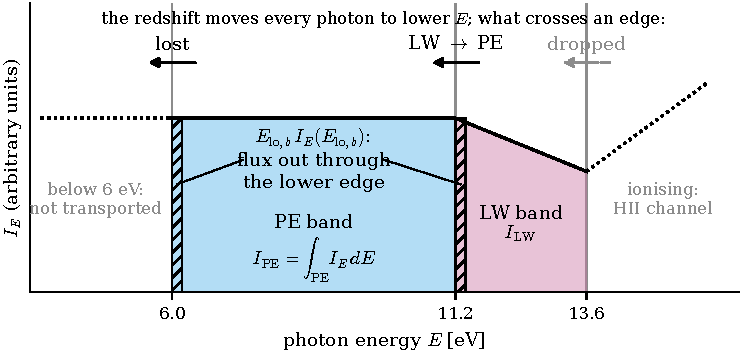
\includegraphics{figures/isrf_band_edge.pdf}
\caption{Band-edge transfer by the redshift, on a sketched spectrum $I_E$
with the default weights. Every photon moves to a lower energy. A band loses
the energy of its photons and the flux $E_{\rm lo}I_E(E_{\rm lo})$ through its
lower edge (hatched). LW feeds PE through $11.2$\,eV; PE loses light below
$6$\,eV; nothing enters LW from above $13.6$\,eV.}
\label{fig:isrf-redshift}
\end{figure}

\subsubsection{Moments and limits}
\label{sec:isrf-rte-limits}

The energy density and the flux of band $b$ are the moments
\begin{equation}
  u_b = \frac{1}{c}\oint I_b\,d\Omega, \qquad
  \boldsymbol{F}_b = \oint I_b\,\boldsymbol{n}\,d\Omega .
  \label{eq:isrf-moments}
\end{equation}
The rates of Eqs.~\eqref{eq:isrf-G0} and \eqref{eq:isrf-kdiss} need the light
from all directions, $c\,u_b=\oint I_b\,d\Omega$, not the net flux: two equal
beams from opposite sides heat twice as much as one, while their net flux is
zero. The specific energy is $\tilde u_b=u_b/\rho$. The scheme does not solve
the moment equations; it transports the intensity in a few directions, and
forms $u_b$ at the end.

\paragraph{Optically thin limit.} In steady state, one star in a static box
gives
\begin{equation}
  c\,u_b(r) = \frac{L_b}{4\pi r^2}\,e^{-\tau_b(r)},
  \qquad \tau_b(r)=\int_0^r\kappa_b\,dr',
  \label{eq:isrf-thin}
\end{equation}
and for $\tau_b\ll1$ the field falls as $r^{-2}$. Here $c\,u_b=|\boldsymbol{F}_b|$,
because all the light moves away from the star. In an expanding box, along a
ray of physical length $\ell$, the light also loses the factor
$e^{-\lambda_E(b)H\ell/c}$, and PE gains part of what LW loses.

\paragraph{Optically thick limit.} The equation has no scattering, so there is
no diffusion limit. In gas with $\kappa_b\ell\gg1$ the light is absorbed
within a few $1/\kappa_b$ of where it enters, and the field behind falls as
$e^{-\tau_b}$ along each ray. A dense cloud casts a sharp shadow.
Section~\ref{sec:isrf-accuracy} shows both limits in a run of the scheme.

\paragraph{Time dependence.} A front of real light moves at $c$. It crosses
$100$\,pc in $330$\,yr, which is short against the dynamical times of the
gas. For the gas the true field is close to its steady state, and the time
derivative matters only during the transient after a star is born or dies.
The scheme moves the light more slowly (Section~\ref{sec:isrf-rte-scope}), so
in the scheme this transient lasts much longer.

\subsubsection{What is kept and what is dropped}
\label{sec:isrf-rte-scope}

Table~\ref{tab:isrf-scope} lists the terms. The speed of the light needs a
word. The equation has $1/c$ in front of the time derivative. The scheme moves
the light at a reduced speed, set by the time step of the gas and by a limit
speed $v\le c$ (Section~\ref{sec:isrf-speed}); with the default settings it is
far below $c$. The field that the gas sees is still formed with the true $c$
(Section~\ref{sec:packet-field}): the scheme carries the flux of the light and
converts it to the energy density that light of that flux has at $c$. A slow
front therefore delays the field but does not scale it. Behind the front the
measured field is 0.90 to 0.95 of the thin limit. Where the light of several
sources shares a slot, $G_0$ of a single particle can differ by up to 13 per
cent from the sum of the sources
(Sections~\ref{sec:isrf-accuracy}, \ref{sec:packet-superposition}). The
approach to the steady field is slower than for real light. The dust
absorption and the redshift are booked per unit of path, not per unit of
time, so a slow front does not change them.

\begin{table}[htbp]
\centering
\caption{The terms of Eq.~\eqref{eq:isrf-rte-solved}: what the scheme keeps
and what it drops.}
\label{tab:isrf-scope}
\begin{tabular}{>{\raggedright\arraybackslash}p{4.6cm}>{\raggedright\arraybackslash}p{9.6cm}}
\toprule
term & treatment \\
\midrule
emission $a^3j_b$ & kept: stars as points, isotropic, $L_b$ constant over the
  feedback step of the star; photon number from the mean photon energy of
  the spectrum \\
dust absorption $\kappa_b\hat I_b$ & kept: grey in each band, $\kappa_b$ of the
  receiving particle, from its density and metallicity \\
free streaming $\boldsymbol{n}\cdot\nabla$ & kept: straight lines from an
  origin, with $K=12$ direction cells per particle (Section~\ref{sec:isrf-idea}) \\
time derivative $\partial_t/c$ & kept with a reduced speed
  (Section~\ref{sec:isrf-speed}) \\
dilution by expansion & kept exactly: the scheme carries energy, not energy
  density, in comoving coordinates \\
redshift $\lambda_E(b)H/c$ & kept, with constant band-edge weights \\
band-edge gain $\hat G_{\rm PE}$ & kept \\
inflow into LW above $13.6$\,eV & dropped: no ionising photons in this channel \\
scattering by dust & dropped: absorption only \\
emission by dust or gas in the bands & dropped \\
H$_2$ line absorption & dropped from the transport: Grackle applies H$_2$
  self-shielding locally \\
redistribution inside a band & dropped: one $\kappa_b$ per band, constant
  $\lambda$ \\
terms of order $u/c$ of the peculiar flow & dropped: Doppler shift and
  aberration (Section~\ref{sec:packet-frame}) \\
heating by the absorbed light & not applied: the gas is heated through $G_0$
  only \\
\bottomrule
\end{tabular}
\end{table}

\paragraph{Why these terms may be dropped.} Dust re-emits what it absorbs in
the infrared, outside the two bands. The redshift depth over $10$\,kpc is
$\zeta\approx4\times10^{-5}$ at $z=9$, and less later. With
$\lambda_E({\rm LW})\approx6.5$ the whole redshift loss over such a path is
below $3\times10^{-4}$, so an error in the constant band-edge weights changes
the field inside a galaxy by less than that. The errors from dropping scattering and the emission of the gas
in the bands, and from one grey opacity per band, have not been estimated.

{\small
\begin{longtable}{>{\raggedright\arraybackslash}p{2.4cm}>{\raggedright\arraybackslash}p{4.4cm}>{\raggedright\arraybackslash}p{7.4cm}}
\caption{Symbols of the transfer equation.}
\label{tab:isrf-rte-symbols}\\
\toprule
symbol & units & meaning \\
\midrule
\endfirsthead
\toprule
symbol & units & meaning \\
\midrule
\endhead
$E$ & erg & photon energy, seen by a comoving observer \\
$I_E$ & erg\,s$^{-1}$\,cm$^{-2}$\,sr$^{-1}$\,erg$^{-1}$ & specific intensity per unit photon energy \\
$I_b$ & erg\,s$^{-1}$\,cm$^{-2}$\,sr$^{-1}$ & intensity of band $b$, $\int_b I_E\,dE$ \\
$\hat I_b$ & erg\,s$^{-1}$\,cm$^{-2}$\,sr$^{-1}$ & $a^3I_b$, intensity of a comoving volume \\
$N_b$, $\hat{\mathcal N}_b$ & photons\,s$^{-1}$\,cm$^{-2}$\,sr$^{-1}$; as $I_b$ & photon-number intensity of band $b$; $a^3E_{{\rm lo},b}N_b$ \\
$b$ & -- & band, PE ($6.0$ to $11.2$\,eV) or LW ($11.2$ to $13.6$\,eV) \\
$E_{{\rm lo},b}$, $E_{{\rm hi},b}$ & erg & lower and upper edges of band $b$ \\
$\boldsymbol{x}$, $\boldsymbol{n}$ & cm, -- & position (comoving in an expanding box) and unit direction \\
$t$, $c$ & s, cm\,s$^{-1}$ & cosmic time and speed of light \\
$a$, $H$ & --, s$^{-1}$ & scale factor ($1$ in a static box) and Hubble rate $\dot a/a$ ($0$ in a static box) \\
$j_E$, $j_b$ & erg\,s$^{-1}$\,cm$^{-3}$\,sr$^{-1}$(\,erg$^{-1}$) & emissivity per unit energy, and of band $b$ \\
$L_{b,\star}$ & erg\,s$^{-1}$ & band luminosity of a star \\
$\kappa_E$, $\kappa_b$ & cm$^{-1}$ & linear absorption coefficient, physical; per energy and per band \\
$\sigma_{{\rm d},b}$ & cm$^2$ & dust cross-section per hydrogen nucleon in band $b$ \\
$\mathcal D(Z)$ & -- & dust-to-gas ratio relative to the Milky Way \\
$Z$, $Z_\odot$ & -- & metal mass fraction of the gas, and the solar value of Grackle \\
$f_{\rm dg}$, $f_{{\rm dg},0}$ & -- & dust-to-gas mass ratio of Grackle, and its default \\
$\mu_{\rm H}$, $m_{\rm H}$ & --, g & mass per hydrogen nucleon in units of $m_{\rm H}$, and the proton mass \\
$\rho$ & g\,cm$^{-3}$ & physical gas density \\
$\lambda_E(b)$, $\lambda_N(b)$ & -- & band-edge weights of the energy and of the photon number \\
$\hat G_b$ & as $\hat I_b$ & gain of band $b$ through its upper edge \\
$\bar E_b$ & erg & mean photon energy of band $b$ \\
$u_b$, $\tilde u_b$ & erg\,cm$^{-3}$, erg\,g$^{-1}$ & energy density of band $b$, and specific energy $u_b/\rho$ \\
$\boldsymbol{F}_b$ & erg\,s$^{-1}$\,cm$^{-2}$ & flux of band $b$ \\
$\tau_b$ & -- & optical depth of band $b$ \\
$G_0$, $F_{\rm H}$ & --, erg\,s$^{-1}$\,cm$^{-2}$ & field strength in Habing units, and the Habing flux \\
$\Gamma_{\rm pe}$, $\epsilon_{\rm pe}$ & erg\,s$^{-1}$, -- & photoelectric heating rate per hydrogen atom, and its efficiency \\
$F_{\rm LW}$ & erg\,s$^{-1}$\,cm$^{-2}$ & LW energy flux from all directions, $c\,u_{\rm LW}$ \\
$\Omega$ & sr & solid angle \\
$\boldsymbol{x}_\star$ & cm & position of a star \\
$r$, $\ell$ & cm & distance to a star; physical length of a ray, or the local attenuation length without transport \\
$k_{\rm diss}$ & s$^{-1}$ & H$_2$ photodissociation rate per molecule \\
$\sigma_{\rm H_2}/\bar E_{\rm LW}$ & cm$^2$\,erg$^{-1}$ & H$_2$ dissociation cross-section over the mean LW photon energy \\
\bottomrule
\end{longtable}
}

% ---------------------------------------------------------------------------
\subsection{The idea of the scheme}
\label{sec:isrf-idea}

Figure~\ref{fig:isrf-overview} shows the steps below in one picture.

\paragraph{Light is carried by the gas.} The scheme has no grid and no
photons of its own. Each gas particle holds the light that is passing through
it, as a few packets. A packet is an amount of energy and of photon number in
each band, with one direction of travel and one distance back to where the
light came from (its origin). The light moves by being handed from one gas
particle to its neighbours.

\paragraph{Twelve reception slots.} The light that crosses a particle comes from
many directions. The particle sorts it by direction into $K=12$ reception
slots. The slots are the cells of a fixed partition of the sphere of
directions into twelve equal cones (the faces of a rhombic dodecahedron). The
frame of this partition is the same for all particles and all steps. Each slot
holds one packet: the light that travels in its range of directions. Twelve
slots are the angular resolution of the scheme. Two directions in one slot are
at most $90^\circ$ apart, so light from opposite sides of a particle never
shares a slot there.

\paragraph{Emission by a star.} At each of its feedback steps, a star hands
the light of that step, $L_b\Delta t_\star$ per band, to the gas particles in
its kernel. To keep the emission isotropic, the star sorts its neighbours into
twelve emission cells of equal solid angle (HEALPix pixels). These emission
cells are not the reception slots. Their frame is a random rotation, drawn
anew for each star and each step. A cell that holds too little gas lets its
part of the light escape. Each receiver gets a share of the light, and puts it
into the reception slot of its direction from the star.

\paragraph{The hop.} Once per own step, each gas particle sends the light of
each slot downstream. The light of a slot goes to the neighbours that lie
ahead along the direction of the slot. A neighbour at angle $\theta$ to that
direction gets a weight $\propto\cos^p\theta$ ($p=4$ by default), times its
volume and the kernel. These weights form a cone of transmission. The particle
keeps nothing: all the light of the slot leaves. Each receiver puts its share
into the slot that holds the direction from the origin of the light to the
receiver. So the light keeps going in a straight line away from its source,
even after many hops.

\paragraph{Absorption and redshift on the way.} The light of a share travels
from the sender to the receiver. The extra distance from the origin, receiver
minus sender, is the path of the share. On delivery, the receiver books the
redshift over this path (in an expanding box) and the dust absorption over it,
with its own $\kappa_b$. Both are exponentials over the path. In uniform gas,
at fixed $a$ and $H$, and with one share per merge, many short hops therefore
give the same energy as one long one (the PE gain to first order in the
redshift). What dust absorbs is booked in a ledger of the receiver.

\paragraph{The merge.} At its next step, each particle collects the light that
has arrived in each slot since its last step, and makes it one packet. The
energy and the photon number add. The new direction and origin distance are
the energy-weighted mean of the origins of the arrivals. Here the scheme loses
the spread of directions inside a slot. The hop cone, the far arrival cells
and the kernel mean of the field below also smooth the light;
Section~\ref{sec:isrf-accuracy} gives the measured sizes.

\paragraph{Time.} Particles have different time steps, and light has a finite
speed. Each share therefore carries an arrival time: the time at which its
light reached the sender, plus the distance over the limit speed $v$. A share
that has not yet arrived waits at the receiver, in one of a few stores per
slot: $N_{\rm n}$ near bins (8 by default), one receiver step wide each, and
two far cells, many steps wide, for the light that arrives later. At each merge the receiver takes
only the light that has arrived. Light from a sender with a longer step is
spread evenly over that step, so a fine receiver does not get it all at once.

\paragraph{The field the gas sees.} A packet is the light that crosses the
particle during one step. Its energy, divided by the mass of the particle and
multiplied by the hop speed over $c$, is the specific energy of that light.
The hop speed is the advance of the light in one hop over the step of the
particle.
The particle sums this over its slots, takes a kernel mean with its
neighbours, and passes the result to Grackle as $G_0$ and $k_{\rm diss}$.

\paragraph{Nothing is lost unaccounted.} Every unit of energy that a star emits
is at any time in one of a few places. It is in flight, absorbed by dust,
removed by the redshift, or escaped from the gas. Or it was removed with a gas
particle that became a star or entered a sink. In a diagnostic build, each
gas particle and each star carries ledgers of these amounts, and their sum
equals the emitted energy to rounding.

\begin{figure}[htbp]
\centering
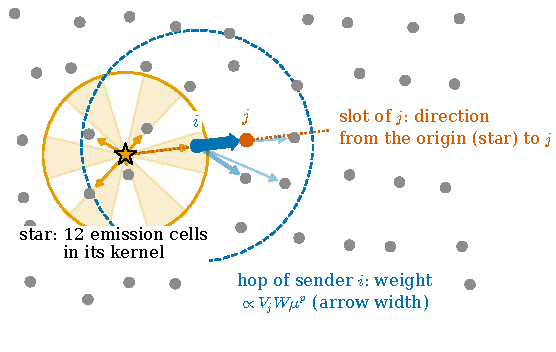
\includegraphics{figures/isrf_overview.pdf}
\caption{The scheme, sketched in two dimensions. The star gives its light
to the gas in its kernel (orange arrows), over twelve emission cells drawn
anew at each step. The sender $i$ hands the light of one slot to the
neighbours ahead (blue, width $\propto$ share). The receiver
$j$ files its share by the direction from the star to $j$.}
\label{fig:isrf-overview}
\end{figure}

% ---------------------------------------------------------------------------
\subsection{From the equation to the scheme}
\label{sec:isrf-discrete}

Table~\ref{tab:isrf-map} maps each term of Eq.~\eqref{eq:isrf-rte-solved} to
a step of the scheme. The packet represents the intensity in the following
sense. Slot $k$ of a particle holds $E_{k,b}$, the energy of band $b$ that
crosses the particle in one step, in the directions of cell $k$. Its photon
number $N_{k,b}$ is the same for the photon-number intensity. The subsections
below give each step. Lengths are comoving unless marked physical; a physical
length is $a$ times the comoving one. Dust absorption, the redshift of the
light, the step lengths and the field that the gas sees are physical.

\begin{longtable}{>{\raggedright\arraybackslash}p{3.6cm}>{\raggedright\arraybackslash}p{7.4cm}>{\raggedright\arraybackslash}p{3.2cm}}
\caption{The terms of Eq.~\eqref{eq:isrf-rte-solved} and the steps of the
scheme that solve them.}
\label{tab:isrf-map}\\
\toprule
term & step of the scheme & subsection \\
\midrule
\endfirsthead
\toprule
term & step of the scheme & subsection \\
\midrule
\endhead
$a^3 j_b$ & star hands $L_b\Delta t_\star$ to its kernel neighbours over 12 emission cells & \ref{sec:packet-emission} \\
$\boldsymbol{n}\cdot\nabla_{\!x}\hat I_b/a$ & hop of each slot down a cone of weights; receiving slot set by the direction from the origin & \ref{sec:packet-state}, \ref{sec:packet-hop} \\
angular structure of $\hat I_b$ & 12 slots, one mean direction each, merged at each step & \ref{sec:packet-merge} \\
$\partial_t\hat I_b/c$ & one hop per step; arrival time with the limit speed $v$; near bins and far cells & \ref{sec:packet-lightspeed}, \ref{sec:packet-reservoir} \\
$-\kappa_b\hat I_b$ & absorption of a share at delivery, over its path & \ref{sec:packet-absorption} \\
$-\lambda_E(b)H\hat I_b/c$, $H\hat G_b/c$ & redshift and band-edge transfer of a share at delivery, over its path & \ref{sec:packet-transfer} \\
$u_b$, Eq.~\eqref{eq:isrf-moments} & sum over the slots, with the hop speed over $c$, then a kernel mean & \ref{sec:packet-field} \\
photon number & carried and treated like the energy & all \\
\bottomrule
\end{longtable}

\subsubsection{Symbols of the scheme}
\label{sec:packet-symbols}

Bands are $b\in\{{\rm PE},{\rm LW}\}$. Slots are numbered by $k$, sending
particles by $i$, receiving particles by $j$, arriving shares by $s$. Two
letters have a second meaning: $H$ is the Hubble rate and $H_{ij}$ a smoothing
length; $\mu$ is a cosine and $\mu_{\rm H}$ a mass per hydrogen nucleon.
Upper-case $E$ and $N$ belong to a slot, lower-case $e$ and $n$ to one share.

\begin{longtable}{p{1.9cm}p{3.4cm}p{8.6cm}}
\caption{Symbols of the scheme.}
\label{tab:packet-symbols}\\
\toprule
symbol & units & meaning \\
\midrule
\endfirsthead
\toprule
symbol & units & meaning \\
\midrule
\endhead
$E_{k,b}$ & energy & band energy held in slot $k$ of a particle \\
$N_{k,b}$ & energy & photon number of slot $k$, stored as $N E_{{\rm lo},b}$ (number of photons times the lower edge energy) \\
$\bar E_b$ & energy & mean photon energy of the band, $E_{{\rm lo},b}\,E_{k,b}/N_{k,b}$ \\
$f_b$ & -- & photon number per unit energy of a star, $E_{{\rm lo},b}/\bar E_b$ \\
$K$ & -- & number of reception slots, 12 by default \\
$\boldsymbol{n}_k$ & -- & unit direction of travel of slot $k$ \\
$d_k$ & length & distance from the origin of slot $k$ to the particle \\
$\boldsymbol{o}$ & length & offset from a particle to the origin of a packet \\
$\boldsymbol{\Delta x}_{ij}$ & length & vector from sender $i$ to receiver $j$ \\
$h_i$ & length & smoothing length of sender $i$; kernel support $\gamma h_i$ \\
$H_{ij}$ & length & $\max(h_i,h_j)$, the length of the kernel in the weight of sender $i$ and receiver $j$ \\
$W,\gamma$ & length$^{-3}$, -- & hydro kernel of the build and its support in units of $h$ \\
$p$ & -- & power of the hop cone, default 4 \\
$\mu_{ij,k}$ & -- & cosine between $\boldsymbol{\Delta x}_{ij}$ and $\boldsymbol{n}_k$ \\
$V_j$ & length$^3$ & comoving volume $m_j/\rho_j$ of receiver $j$ \\
$w_{ij,k}$ & -- & hop weight of slot $k$ towards $j$ \\
$S_{i,k}$ & -- & sum of the hop weights of slot $k$ over the neighbours of $i$ \\
$l_{i,k}$ & length & mean advance of slot $k$ of sender $i$ along its direction \\
$\kappa_b$ & 1/length & linear dust absorption rate of band $b$ at the receiver, physical (Eq.~\eqref{eq:isrf-kappa}) \\
$\lambda_E(b)$, $\lambda_N$ & -- & band-edge weight of the energy of band $b$, and of the LW photon number (Eqs.~\eqref{eq:isrf-lambdaE}, \eqref{eq:isrf-lambdaN}) \\
$H$, $\zeta$ & 1/time, -- & Hubble rate, and redshift depth of a share, $\zeta=H\,\ell_{\rm phys}/c$ \\
$\ell_{\rm phys}$ & length & physical path length of a share, $\ell_{\rm phys}=a\,\Delta\ell$ \\
$\nu$ & -- & rate per unit $\zeta$ at which the PE photon number crosses $6$\,eV \\
$R$ & -- & rotation matrix of the slot frame \\
$L_b$ & energy/time & band luminosity of a star, physical \\
$\Delta t_\star$ & time & feedback step of the star, proper time \\
$m_j$, $\rho_j$ & mass, mass/length$^3$ & mass and (comoving) density of gas particle $j$ \\
$a$ & -- & scale factor, 1 in a static box \\
$v$, $f$ & length/time, -- & limit speed of the light, $v=fc$ \\
$P_{\beta,k,b}$, $g_\beta$ & energy, -- & light of band $b$ waiting in store $\beta$ of slot $k$, and the fraction of it released at a merge \\
$O_k$, $E_{\rm wait}$ & energy$\times$length, energy & origin sum $\sum_s e_s\boldsymbol{o}_s$ of the waiting light of slot $k$, and its energy \\
$f_{{\rm rel},k}$ & -- & fraction of the reservoir of slot $k$ released at a merge \\
$B_{k,b}$ & energy & reservoir of slot $k$ (light from sources with a longer step) \\
$t_{{\rm d},i}$ & time & departure time of the held packet of sender $i$: its merge time, the end of its step minus its step \\
$S_{\rm floor}$ & length$^3$ & cell floor of a star's emission \\
$E_{\rm fl}$ & energy & light in flight \\
$A$, $X$, $Y$ & energy & cumulative absorbed, escaped and redshift ledgers of a gas particle \\
$E_{\rm rm}$, $E_{\rm inh}$ & energy & removed and inherited ledgers of a star or a sink \\
\bottomrule
\end{longtable}

\subsubsection{The packet and its reception slots}
\label{sec:packet-state}

A gas particle holds one packet per reception slot. The slots are the cells of a
partition of the sphere of directions into $K$ cells of equal solid angle. The
cells are convex cones fixed in a rotated frame, so the mean of any set of
directions of one cell lies in that cell. Each slot holds, for both bands, the
energy $E_{k,b}$ and the photon number $N_{k,b}$, and for both bands together
one direction $\boldsymbol{n}_k$ and one distance $d_k$ to its origin. The mean photon energy
of a band follows from the pair,
\begin{equation}
  \bar E_b = E_{{\rm lo},b}\,\frac{E_{k,b}}{N_{k,b}}.
  \label{eq:packet-meanE}
\end{equation}
A star sets the photon number of its emission from the mean photon energy
of its spectrum in the band, clamped to the band,
\begin{equation}
  N = f_b\,E, \qquad f_b=\frac{E_{{\rm lo},b}}{\bar E_b}, \qquad
  E_{{\rm lo},b}\le \bar E_b\le E_{{\rm hi},b}.
  \label{eq:packet-photonfrac}
\end{equation}

\paragraph{The slot function.} Let $\boldsymbol{y}=R\,\boldsymbol{x}$ be a
direction $\boldsymbol{x}$ in the frame, $R$ a rotation matrix. The slot of
a direction depends on the number $K$ of slots, a compile-time option.
\begin{align}
  K=8:&\quad k=\sum_{m=0}^{2} 2^m\,[\,y_m\ge 0\,], \label{eq:packet-slot8}\\
  K=12:&\quad k=4m+2\,[\,y_{m_1}\ge0\,]+[\,y_{m_2}\ge0\,], \quad
  m=\arg\min_{m'} |y_{m'}|, \label{eq:packet-slot12}\\
  K=16:&\quad k=\sum_{m=0}^{2} 2^m\,[\,y_m\ge 0\,]+8\,[\,|y_1|>|y_0|\,],
  \label{eq:packet-slot16}\\
  K=24:&\quad k=4(2m+s)+2t+b, \label{eq:packet-slot24}\\
  K=48:&\quad k=8(2m+s)+4t+2b+c, \label{eq:packet-slot48}
\end{align}
with $[\cdot]$ equal to 1 if the condition holds and 0 otherwise. In
Eqs.~\eqref{eq:packet-slot24} and~\eqref{eq:packet-slot48}, $m$ is the axis of
the largest $|y|$ (the lowest axis on a tie), $s=[\,y_m\ge0\,]$, $(m_1,m_2)$
are the two other axes in axis order, $t=[\,|y_{m_1}|\ge|y_{m_2}|\,]$, and $b$
and $c$ are $[\,y\ge0\,]$ for the larger and for the smaller of $|y_{m_1}|$ and
$|y_{m_2}|$. In
Eq.~\eqref{eq:packet-slot12}, $m$ is the axis of the smallest $|y|$, the
lowest axis on a tie. The indices $(m_1,m_2)$ are the two other axes in axis
order: $(1,2)$ for $m=0$, $(0,2)$ for $m=1$ and $(0,1)$ for $m=2$. For $K=8$
the cells are the octants of the frame. For $K=12$ they are the faces of a
rhombic dodecahedron (Fig.~\ref{fig:isrf-slots}). For $K=16$ they are the octants halved by the plane
$|y_0|=|y_1|$; a tie $|y_0|=|y_1|$ goes to the lower half. For $K=24$ and $48$
the cells are the faces of a tetrakis hexahedron and of a disdyakis
dodecahedron (Sec.~\ref{sec:isrf-code}). A direction on a
border goes to the cell with the positive coordinate, whatever the sign of a
zero. A direction in the same octant as another differs from it by at most
$90^\circ$. The cells of $K=16$ lie inside octants, and those of $K=12$ also
keep two directions within $90^\circ$: in a cell with $|y_m|\le y_{m_1}$ and
$|y_m|\le y_{m_2}$, the dot product of two unit vectors is at least
$y_{m_2}y'_{m_2}\ge0$. For every $K$, the opposite direction $-\boldsymbol y$
flips the signs that select the cell, so it falls in another slot unless it
lies on a border.

\begin{figure}[htbp]
\centering
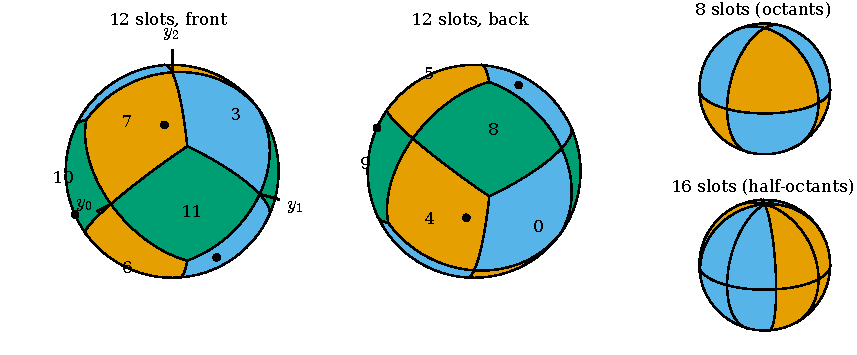
\includegraphics{figures/isrf_slots.pdf}
\caption{The reception slots on the sphere of directions, in the slot frame
$(y_0,y_1,y_2)$. Left: the 12 slots, front and back, coloured by the axis $m$
of Eq.~\eqref{eq:packet-slot12} and numbered by $k$: convex cones of equal
solid angle. Dots: the box axes, each at least $10^\circ$ from a border.
Right: 8 and 16 slots (octants, halved octants).}
\label{fig:isrf-slots}
\end{figure}

\paragraph{The frame.} The matrix is
\begin{equation}
  R = R_z(\theta_z)\,R_y(\theta_y)\,R_x(\theta_x),
  \label{eq:packet-frame}
\end{equation}
with $\theta_x,\theta_y,\theta_z$ three run-time angles, default
$(24^\circ,36^\circ,66^\circ)$. The default keeps every cell border at least
$10^\circ$ from the six box axes for $K=12$ ($19^\circ$ for $K=8$, $6^\circ$
for $K=16$, $24$ and $48$). Box diagonals can lie on a border: the $(1,1,1)$ directions are
$0.01^\circ$ from one at $K=12$. A source or beam exactly along a box diagonal
then gets an arbitrary but deterministic slot; rotate the frame for such a
setup. A positive run-time seed offset multiplies $R$ on the left by a rotation drawn uniformly from that seed
\citep{Shoemake1992}, so that repeats of a run use independent frames. The
frame is the same for every particle.

\subsubsection{The hop}
\label{sec:packet-hop}

Once per own step, every active sender $i$ hands the energy and the photon
number held in each non-empty slot $k$ to its neighbours. Slot $k$ sends to
neighbour $j$ the fraction
\begin{equation}
  \phi_{ij,k} = \frac{w_{ij,k}}{S_{i,k}}, \qquad
  S_{i,k}=\sum_{j'} w_{ij',k}, \qquad
  w_{ij,k}=V_j\,W(r_{ij},H_{ij})\,\mu_{ij,k}^{\,p},\qquad
  H_{ij}=\max(h_i,h_j),
  \label{eq:packet-share}
\end{equation}
where $r_{ij}=|\boldsymbol{\Delta x}_{ij}|$ and
$\mu_{ij,k}=\boldsymbol{\Delta x}_{ij}\!\cdot\!\boldsymbol{n}_k/r_{ij}$. The
sum $S_{i,k}$ is the SPH quadrature of $\int W\mu^p\,\mathrm{d}V$, so across a
density gradient the shares follow the solid angle and not the number of
neighbours on each side. The density in $V_j$ is the value of the previous
step, so the sum $S_{i,k}$ and the shares use the same weights; its expansion
factor is common to all receivers and cancels in $\phi_{ij,k}$. The weight
$w_{ij,k}$ is zero if $r_{ij}=0$, if $j$ is not in the reach of $i$
(Section~\ref{sec:isrf-reach}), or if $\mu_{ij,k}\le\mu_{\rm min}=10^{-3}$.
The cut at $\mu_{\rm min}$ removes the neighbours behind and beside the
sender; a neighbour just above it has a weight of order
$\mu_{\rm min}^p$ times that of one straight ahead, $10^{-12}$ at $p=4$, so
the cut moves no measurable light. The sum runs over all neighbours with non-zero weight, so
$\sum_j\phi_{ij,k}=1$ up to float rounding. The hop hands on the whole of each
slot: nothing is kept by the sender.

\paragraph{One weight per pair.}
The shares of a sender sum to one only if the sender loop, which builds
$S_{i,k}$, and the receiver loop, which builds $\phi_{ij,k}=w_{ij,k}/S_{i,k}$,
evaluate the same $w_{ij,k}$ for every pair. A pair vector formed in the local
frame of each loop's cell differs between the two loops by float rounding.
Near the kernel edge $W$ and $\mu^{p}$ vary steeply, so that rounding gives two
different weights. Then $\sum_j\phi_{ij,k}\ne1$ and light is created or lost.
For the cell frames tested, the two frames disagreed on the weight of 21 to 46
percent of pairs. Both loops therefore form $\boldsymbol{\Delta x}_{ij}$ from
the absolute positions in double precision, wrapped to the nearest periodic
image, and the weight is identical for the pair, also across a periodic face.
This vector fixes the value of the weight only. It does not select which
neighbours are visited (Section~\ref{sec:isrf-code}).

For the Wendland-C2 kernel used in GEAR runs (three dimensions),
\begin{equation}
  W(r,h) = \frac{21}{2\pi\,\gamma^{3}h^{3}}\,(1-q)^4\,(1+4q), \qquad
  q=\frac{r}{\gamma h},\quad \gamma=1.936492,
  \label{eq:packet-kernel}
\end{equation}
which is the polynomial $4q^5-15q^4+20q^3-10q^2+1$, equal to $(1-q)^4(1+4q)$
\citep{Wendland1995}. Other kernels give their own $W$. The constant
$21/(2\pi\gamma^3)$ is the same for every neighbour of $i$ and cancels in
$\phi_{ij,k}$. The factor $H_{ij}^{-3}$ does not cancel: it is $h_i^{-3}$ for
a neighbour with $h_j\le h_i$, and $h_j^{-3}$ for a neighbour with a larger
smoothing length, whose kernel is then also evaluated at $r_{ij}/h_j$. In gas
of uniform smoothing length it is common to all neighbours. A larger $p$ gives
a narrower cone.

The share is placed in the slot of the receiver that holds the direction from
the packet's origin to the receiver (Fig.~\ref{fig:isrf-hop}a). Seen from the receiver, the origin lies at
\begin{equation}
  \boldsymbol{o}_{j} = -\boldsymbol{\Delta x}_{ij} - d_{i,k}\,\boldsymbol{n}_{i,k},
  \label{eq:packet-offset}
\end{equation}
because the origin is $d_{i,k}$ behind the sender along its direction. The
slot of the receiver is the slot function of
Eqs.~\eqref{eq:packet-slot8}--\eqref{eq:packet-slot48} applied to
$-\boldsymbol{o}_j$. The slot is chosen from this geometry and not from the
slot index of the sender. The share carries the energy $\phi_{ij,k}E_{i,k,b}$
and the photon number $\phi_{ij,k}N_{i,k,b}$ of each band $b$, changed by the
redshift and the band-edge transfer of Section~\ref{sec:packet-transfer} and
reduced by the absorption of Section~\ref{sec:packet-absorption}.

\begin{figure}[htbp]
\centering
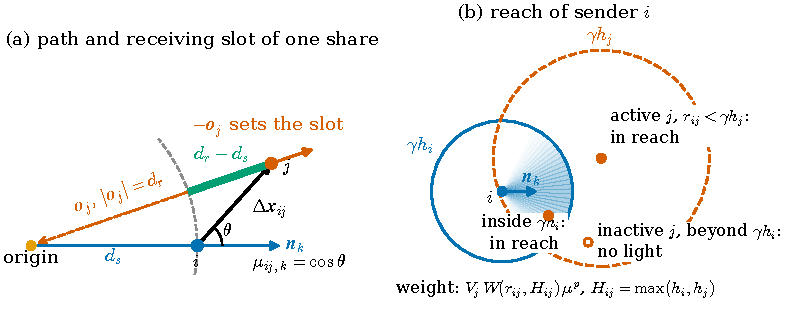
\includegraphics{figures/isrf_hop.pdf}
\caption{(a) One share of a hop. The receiver $j$ books dust and redshift
over the path $d_r-d_s$ (green). The
direction $-\boldsymbol{o}_j$ from the origin sets the slot of $j$. (b) The
reach of the sender $i$: its own kernel, plus the kernel of an active
receiver. An inactive receiver beyond $\gamma h_i$ gets nothing. Shading:
$\mu^p$.}
\label{fig:isrf-hop}
\end{figure}

Together with $S_{i,k}$ the scheme forms the mean advance of the slot along
its direction,
\begin{equation}
  l_{i,k} = \frac{1}{S_{i,k}}\sum_{j} w_{ij,k}\,
  \boldsymbol{\Delta x}_{ij}\!\cdot\!\boldsymbol{n}_{i,k},
  \label{eq:packet-advance}
\end{equation}
which Section~\ref{sec:packet-field} uses. If a non-empty slot has
$S_{i,k}=0$, it has no downstream neighbour, and its light is booked as escaped
(Section~\ref{sec:packet-ledger}).

\subsubsection{The merge}
\label{sec:packet-merge}

At each active step of the particle, at time $t$ when its previous step has
ended, the light of each slot that has arrived becomes the held packet. Until
then a share waits in a store of the slot. Let $P_{\beta,k,b}$ be the energy
of band $b$ that waits in store $\beta$ of slot $k$, and $g_\beta\in[0,1]$
the fraction of it that is due at $t$. Then
\begin{equation}
  E_{k,b} \leftarrow E_{k,b} + \sum_\beta g_\beta\,P_{\beta,k,b},
  \label{eq:packet-merge-E}
\end{equation}
and the photon number $N_{k,b}$ is updated in the same way, with the same
$g_\beta$. The transport has three modes for the speed of the light
(Section~\ref{sec:packet-lightspeed}). In the default capped mode and in the
step-bounding mode, each slot has the stores of Section~\ref{sec:isrf-idea}:
$N_{\rm n}$ near bins (8 by default), one receiver step wide each, and two far
cells, many steps wide, for light that arrives later. A near bin ends at the
time $T_\beta$ and holds the light that arrives by then; the far cell of a
particle that has not yet merged holds light
that arrives evenly from $t_{{\rm f},\beta}$ to $t_{{\rm l},\beta}$ (a pulse
has $t_{{\rm f},\beta}=t_{{\rm l},\beta}$). The due
fractions are
\begin{equation}
  g_\beta^{\rm near}=\begin{cases}1,&T_\beta\le t,\\0,&T_\beta>t,\end{cases}
  \qquad
  g_\beta^{\rm far}=\begin{cases}
    0,& t\le t_{{\rm f},\beta},\\
    \dfrac{t-t_{{\rm f},\beta}}{t_{{\rm l},\beta}-t_{{\rm f},\beta}},
      & t_{{\rm f},\beta}<t<t_{{\rm l},\beta},\\
    1,& t\ge t_{{\rm l},\beta}.
  \end{cases}
  \label{eq:packet-merge-g}
\end{equation}
A particle that has merged once has a known step, which is every particle
after its first merge. Its far cell also ends at $T_\beta$ and is released
whole, $g_\beta=g_\beta^{\rm near}$. Light that arrives beyond the end of the
last cell widens the cells (Section~\ref{sec:packet-lightspeed}), so it is
released whole at the end of its cell. Light beyond the cells at the widest
width, and light that arrives after the end of the time line, stay in the last
cell as a pulse at their latest arrival time, released by $g_\beta^{\rm far}$
with $t_{{\rm f},\beta}=t_{{\rm l},\beta}$. Faint light that falls beyond the
last cell is released whole at its end.
The third mode, the no-delay test mode, is a limit case with two stores: an
inbox, with $g=1$, and a reservoir $B_{k,b}$, with $g=f_{{\rm rel},k}$
(Section~\ref{sec:packet-reservoir}).

Each share brought an offset $\boldsymbol{o}_s$ to its origin
(Eq.~\eqref{eq:packet-offset}, or the star-to-gas vector of
Section~\ref{sec:packet-emission}) and a transmitted energy
$e_s=\sum_b e_{s,b}$, summed over both bands. The slot keeps the origin sum
$O_k=\sum_s e_s\boldsymbol{o}_s$ of its waiting light and the waiting energy
$E_{\rm wait}=\sum_{\beta,b}P_{\beta,k,b}$. A merge that releases the energy
$E_{\rm rel}=\sum_{\beta,b}g_\beta P_{\beta,k,b}\le E_{\rm wait}$ takes the
same fraction $E_{\rm rel}/E_{\rm wait}$ of the origin sum and divides it by
the released energy. The new origin is (Fig.~\ref{fig:isrf-merge}a)
\begin{equation}
  \boldsymbol{o}_k = \frac{1}{E_{\rm rel}}\,
  \frac{E_{\rm rel}}{E_{\rm wait}}\,O_k = \frac{O_k}{E_{\rm wait}},
  \qquad d_k=|\boldsymbol{o}_k|, \qquad
  \boldsymbol{n}_k = -\frac{\boldsymbol{o}_k}{d_k},
  \label{eq:packet-merge-origin}
\end{equation}
for $d_k>0$: the energy-weighted mean origin of all the light that waited, not
only of the released part. The rest of the sum,
$(1-E_{\rm rel}/E_{\rm wait})\,O_k$, stays with the light that still waits, so
its mean origin is unchanged. For $d_k=0$ the direction is
$\boldsymbol{n}_k=(0,0,1)$. In the no-delay mode the inbox and the reservoir
keep separate origin sums. The merge takes the whole inbox sum and the
fraction $f_{{\rm rel},k}$ of the reservoir sum, so the origin is the mean
over the released light only. One
origin and one direction serve both bands. A slot that received no energy
keeps its origin and direction. The energy held before the merge is not part
of the mean: the slot is empty at the merge, because the hop sent its content.

Every share was placed in its slot by its own geometry, so slots never merge
with each other. Within a slot, the merge conserves the energy and the photon
number of each band exactly (they are sums). It does not conserve the
directions: the individual directions of the arriving shares are replaced by
one mean direction, and the angular spread of the slot is lost. Because
$|\sum e_s\boldsymbol{o}_s|\le\sum e_s|\boldsymbol{o}_s|$, the merged distance
$d_k$ is not larger than the energy-weighted mean of the distances of the
shares. For origins spread over a small angle $\theta$ seen from the
particle, the difference is of order $\theta^2/2$ of the distance. The
redshift and the dust absorption of the later hops are computed from the
merged origin (Sections~\ref{sec:packet-transfer} and
\ref{sec:packet-absorption}), not from the separate paths. The effect of this
on the absorption has not been measured for several shares. The
vectors $-\boldsymbol{o}_s$ all lie in one convex cone. Their positive
combination $-\boldsymbol{o}_k$ lies in that cone too, so the direction
$\boldsymbol{n}_k$ is in the cell of its slot, apart from the case $d_k=0$.

\begin{figure}[htbp]
\centering
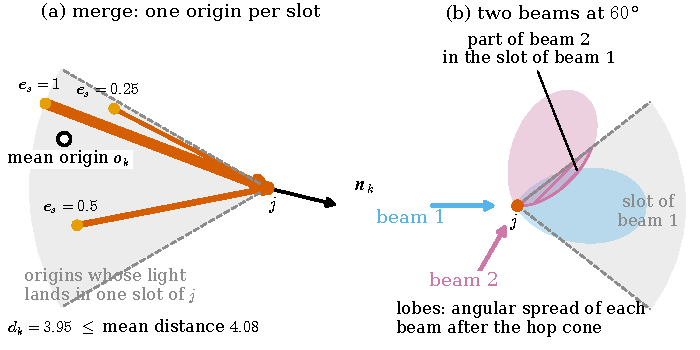
\includegraphics{figures/isrf_merge.pdf}
\caption{(a) The merge: three shares in one slot (width $\propto$ energy)
become one packet with the energy-weighted mean origin (open circle), and a
direction away from it. (b) Two beams at $60^\circ$. The hop cone spreads
each fan beam (lobes); the hatched part of beam 2 ($8.4$ per cent, measured)
merges into the slot of beam 1.}
\label{fig:isrf-merge}
\end{figure}

\subsubsection{Emission by a star}
\label{sec:packet-emission}

A star gives its light of one feedback step, $L_b\Delta t_\star$ per band, to
the gas particles around it. These particles are the receivers: gas with
$q<q_{\rm e}$, where $q=r/(\gamma h_\star)$ is the distance to the star over
the kernel support radius, $q_{\rm e}=0.95$, and a positive density. The
receivers are sorted into $n_c=12$ emission cells, the pixels of a HEALPix map
with \code{nside}$=1$. These cells have equal solid angle $4\pi/12$. Their
frame is a uniform random rotation $Q$ that depends on the ID of the star and
on the start $t_{\rm b}$ of its step, so the cell pattern changes at each step.
With three uniform numbers $u_1,u_2,u_3\in[0,1)$ drawn from a counter-based
generator keyed by the star ID and by $3t_{\rm b}+0$, $+1$, $+2$, the unit
quaternion $(\chi_x,\chi_y,\chi_z,\chi_w)$ is \citep{Shoemake1992}
\begin{align}
  \chi_x&=\sqrt{1-u_1}\,\sin 2\pi u_2, & \chi_y&=\sqrt{1-u_1}\,\cos 2\pi u_2,\nonumber\\
  \chi_z&=\sqrt{u_1}\,\sin 2\pi u_3, & \chi_w&=\sqrt{u_1}\,\cos 2\pi u_3,
  \label{eq:packet-quat}
\end{align}
and the cell $c$ of a gas particle is the pixel \citep{Gorski2005} that
contains $Q\,\hat{\boldsymbol{d}}$, with $\hat{\boldsymbol{d}}$ the unit vector
from the star to the gas.

Each receiver $j$ in cell $c$ has the weight
\begin{equation}
  w_j = \frac{m_j}{\rho_j}\Big(1-\frac{q_j}{q_{\rm e}}\Big),
  \label{eq:packet-tent}
\end{equation}
which is the comoving volume of the particle times a linear (tent) function of
$q$ that falls to zero at $q_{\rm e}$. The weight is zero beyond $q_{\rm e}$, so
a pair near the edge of the support cannot change a share. Let
$S_c=\sum_{j\in c}w_j$ be the weight sum of the cell, and
\begin{equation}
  S_{\rm floor} = f_0\,\frac{\pi}{3}\,\frac{(q_{\rm e}\gamma h_\star)^3}{n_c},
  \qquad f_0=\tfrac12,
  \label{eq:packet-floor}
\end{equation}
the cell floor. $S_{\rm floor}$ is $f_0$ times the value of $S_c$ for a uniform
gas, because $\int_0^{r_{\max}}4\pi r^2(1-r/r_{\max})\,dr=\pi r_{\max}^3/3$ with
$r_{\max}=q_{\rm e}\gamma h_\star$. The floor keeps a lone receiver near the
edge of an almost empty cell from taking the whole twelfth of the light. The
value $f_0=\tfrac12$ is a choice: a cell with at least half the weight of
uniform gas delivers all its light. No measurement fixes it. Each cell holds $1/n_c$ of the star's
light. The part of it that no receiver takes escapes, with the escaping
fraction of cell $c$
\begin{equation}
  \varepsilon_c =
  \begin{cases}
    0, & S_c\ge S_{\rm floor},\\
    (1-S_c/S_{\rm floor})/n_c, & 0<S_c<S_{\rm floor},\\
    1/n_c, & S_c=0.
  \end{cases}
  \label{eq:packet-escape}
\end{equation}
The delivered fraction $D=1-\sum_c\varepsilon_c$ is shared by all receivers of
the star in proportion to their weights: receiver $j$ gets the fraction of the
star's light
\begin{equation}
  \varphi_j = D\,\frac{w_j}{S_{\rm tot}}, \qquad S_{\rm tot}=\sum_c S_c,
  \label{eq:packet-emit-share}
\end{equation}
so $\sum_j\varphi_j=D$. A cell with fewer emitters than its volume needs does
not raise the share of its receivers, because the shares do not depend on the
cell of the receiver. A cell with a real hole ($S_c<S_{\rm floor}$) still lets
its part escape. A star with no receiver loses all its light, $D=0$. The energy
of receiver $j$ in band $b$ is $L_b\Delta t_\star\,\varphi_j$ and its photon
number is $f_b$ times that energy (Eq.~\eqref{eq:packet-photonfrac}). The share
arrives with the offset $\boldsymbol{o}=\boldsymbol{x}_\star-\boldsymbol{x}_j$
of the origin at the star, and it is absorbed along the distance
$r=|\boldsymbol{o}|$ (Section~\ref{sec:packet-absorption}). The cell sums
$S_c$ and the shares use the same weights, so the shares and the escaped
fractions sum to one.

\subsubsection{Redshift and band-edge transfer}
\label{sec:packet-transfer}

This step solves the terms in $H$ of Eq.~\eqref{eq:isrf-rte-solved}. Along a
ray, $c\,dt=d\ell_{\rm phys}$, and the terms in $H$ alone give
$d\hat I_b/d\ell_{\rm phys}=-(H/c)\lambda_E(b)\hat I_b+(H/c)\hat G_b$. A share
loses energy to the expansion along its path. The loss is taken once, when the
share is booked, and before the dust acts (Section~\ref{sec:packet-absorption}).
With $\ell_{\rm phys}$ the physical path of the share
(Eq.~\eqref{eq:packet-path} times $a$), $H$ the Hubble rate and $c$ the speed
of light, the redshift depth is
\begin{equation}
  \zeta = \frac{H\,\ell_{\rm phys}}{c}.
  \label{eq:packet-zeta}
\end{equation}
The energy of the share in LW and PE, before ($e$) and after ($e'$), is
\begin{align}
  e'_{\rm LW} &= e_{\rm LW}\,e^{-\lambda_E({\rm LW})\,\zeta}, \nonumber\\
  e'_{\rm PE} &= e_{\rm PE}\,e^{-\lambda_E({\rm PE})\,\zeta}
    + \frac{\lambda_E({\rm LW})-1}{\lambda_E({\rm LW})}\,
      \big(e_{\rm LW}-e'_{\rm LW}\big).
  \label{eq:packet-redshift-E}
\end{align}
The photon number $n$ of LW (stored as $N E_{\rm lo}$) falls with its own
weight $\lambda_N$, and the photons that it loses enter PE in units of the PE
lower edge. The photon number of PE falls at the rate with which its own
photons cross $6$\,eV, $\nu=(\lambda_E({\rm PE})-1)\,e_{\rm PE}/n_{\rm PE}
=(\lambda_E({\rm PE})-1)\,\bar E_{\rm PE}/E_{{\rm lo},{\rm PE}}$
(Eq.~\eqref{eq:isrf-lambdaN}), $\bar E_{\rm PE}$ being the mean photon energy
of the share:
\begin{align}
  n'_{\rm LW} &= n_{\rm LW}\,e^{-\lambda_N\,\zeta}, \nonumber\\
  n'_{\rm PE} &= n_{\rm PE}\,e^{-\nu\,\zeta}
    + \frac{E_{{\rm lo},{\rm PE}}}{E_{{\rm lo},{\rm LW}}}\,
      \big(n_{\rm LW}-n'_{\rm LW}\big).
  \label{eq:packet-redshift-N}
\end{align}
The LW lines of Eqs.~\eqref{eq:packet-redshift-E} and
\eqref{eq:packet-redshift-N} solve the terms in $H$ exactly. The PE lines are
exact for the PE light already present, but the gain from LW enters without the
PE loss over the same hop. Against the exact solution of
$de_{\rm PE}/d\zeta=-\lambda_E({\rm PE})e_{\rm PE}+(\lambda_E({\rm LW})-1)e_{\rm LW}$,
the gain is too large by the relative amount $\lambda_E({\rm PE})\zeta/2$,
below $10^{-7}$ for a hop of $7$\,pc up to $z=9$
(Section~\ref{sec:packet-frame}).

The scheme computes $\nu$ for each share from its own mean photon energy, so
no table value is needed. The PE photon gain and the PE energy gain describe
the same photons only if the mean photon energy of the share equals that of
the reference spectrum of the weights. Otherwise the PE photon number and the
PE energy drift slowly apart. The PE photon number does not reach Grackle, so
this affects only a ledger. In every
band, the amount removed, net of the gain from the other band, is added to the
redshift ledger $Y$ of the receiver (Section~\ref{sec:packet-ledger}).
$Y_{\rm PE}$ can be negative. At fixed $a$ and $H$, and when each merge receives
a single share, $\zeta$ adds along a chain of hops as the path does. One long
hop and many short hops then give the same LW energy and LW photon number, and
the same PE amounts to first order in $\zeta$. $H$ and $a$ are the values at
the time of the booking, for a hop and for a star. With $H=0$ in a static box,
there is no redshift and no transfer.

\paragraph{Order of redshift and dust.} The scheme applies the redshift first
and the dust second. A combined depth $\tau+\lambda_E\zeta$ gives the same LW
energy; the PE gain and the split between the redshift and absorbed ledgers
differ by order $\zeta\tau E$, below $10^{-7}E$ for $\tau\le1$ and a $7$\,pc
hop up to $z=9$.

\subsubsection{Dust absorption}
\label{sec:packet-absorption}

This step solves the term $-\kappa_b\hat I_b$ of
Eq.~\eqref{eq:isrf-rte-solved}. A share is absorbed by dust along the distance
that its light travelled to the receiver. In an expanding box the redshift of
Section~\ref{sec:packet-transfer} acts first, and the dust acts on what
remains. The dust uses the linear absorption rate $\kappa_b$ of the receiver
in band $b$ (Eq.~\eqref{eq:isrf-kappa}), constant along the path. The receiver
updates $\kappa_b$ from its physical density and its metallicity whenever its
position is updated, active or not, so an inactive receiver uses its last
value. The optical
depth, the absorbed fraction and the transmitted amounts are
\begin{align}
  \tau_b &= \kappa_b\,\ell_{\rm phys} = \kappa_b\,a\,\Delta\ell, \label{eq:packet-tau}\\
  \alpha_b &=
  \begin{cases}
    1-e^{-\tau_b}, & \tau_b<80,\\
    1, & \tau_b\ge 80,
  \end{cases} \label{eq:packet-alpha}\\
  e_{b}^{\rm tr} &= (1-\alpha_b)\,e_b, \qquad
  n_{b}^{\rm tr} = (1-\alpha_b)\,n_b, \label{eq:packet-transmit}
\end{align}
with $e_b$ and $n_b$ the energy and the photon number of the share after the
redshift and before the absorption. The cut at $\tau_b=80$ drops a
transmitted fraction below $e^{-80}\approx1.8\times10^{-35}$, which is
negligible.
Energy and photon number lose the same
fraction, so the mean photon energy of a band is not changed by absorption
(Eq.~\eqref{eq:packet-meanE}). If $n^{\rm tr}_b<10^{-35}$ (internal units of
$N E_{\rm lo}$), the whole share of the band is booked as absorbed and nothing
is transmitted. This keeps the photon number away from the float minimum, where
it would flush to zero before the energy.

The path length is
\begin{equation}
  \Delta\ell =
  \begin{cases}
    \max(0,\,d_r-d_s), & \text{hop from a particle},\\
    r_{\star j}, & \text{emission by a star},
  \end{cases}
  \label{eq:packet-path}
\end{equation}
where $d_s=d_{i,k}$ is the distance from the origin to the sender, and
$d_r=|\boldsymbol{o}_j|$ is the distance from the origin to the receiver,
$\boldsymbol{o}_j$ being the offset of Eq.~\eqref{eq:packet-offset}. For a
star, $d_s=0$ and $d_r=r_{\star j}$. For $\mu_{ij,k}>0$,
$d_r^2=d_s^2+2d_s\,\boldsymbol{\Delta x}_{ij}\!\cdot\!\boldsymbol{n}_{i,k}+r_{ij}^2>d_s^2$,
so the clamp acts only on rounding. When each merge receives a single share,
the merge keeps the origin of that share, and the path lengths add up to the
distance from the origin to the last receiver. The transmitted amounts are
booked into a store of the receiver slot (Section~\ref{sec:packet-merge}),
and the absorbed amounts into the
absorbed ledger of the receiver (Section~\ref{sec:packet-ledger}). The absorbed
energy is a diagnostic: it is not added to the gas, which sees the light only
through the field of Section~\ref{sec:packet-field}.

\subsubsection{A finite speed of light}
\label{sec:packet-lightspeed}

This step solves the time derivative of Eq.~\eqref{eq:isrf-rte-solved} with a
limit speed $v$ in place of $c$.

\paragraph{Modes.} The default capped mode limits the speed of the light to
$v=fc$ (default $f=0.99$) and sets no bound on the time step. The
step-bounding mode also bounds the step of every gas particle
(Section~\ref{sec:isrf-speed}). The no-delay test mode is the limit
$v\to\infty$ (Section~\ref{sec:packet-reservoir}).

\paragraph{Arrival time.} Let $t_{{\rm d},i}$ be the departure time of sender
$i$: the merge time at which it formed its held packet. A share to a
receiver at the comoving separation $r_{ij}$ arrives at
\begin{equation}
  t_{\rm a}=t_{{\rm d},i}+\frac{a\,r_{ij}}{v-\max(0,u_{j})},
  \label{eq:packet-arrival}
\end{equation}
with $u_j$ the peculiar velocity of the receiver along
$\boldsymbol{\Delta x}_{ij}$ at the booking: the front must catch up with a
receiver that moves away. The factor $v/(v-u_j)$ is capped at 100, so the delay
stays finite for a receiver that recedes at nearly $v$; such a receiver gets
its light early (Section~\ref{sec:isrf-speed}). The value 100 is a choice. The
delay is measured from the merge time, so a hop never starts before the sender
has released its light. The receiver releases the light at the end of its near
bin or far cell, which is at or after the arrival; the front of a chain of
particles therefore lags the light time by the sum of the waits at the hops
(below). In an expanding box the time
variable is $\ln a$, and the delay $a\,r_{ij}/v$ becomes the increment
$H\,a\,r_{ij}/v$ of $\ln a$, with $H$ at the booking.

\paragraph{Arrival bins and cells.} A share arrives evenly between $t_{\rm a}$
and $t_{\rm a}+\Delta t_s$ if its sender has a longer step $\Delta t_s$, and
at $t_{\rm a}$ otherwise. A star applies its feedback at the end $t$ of its step
$\Delta t$, and spreads the light of the step from $t-\Delta t+\delta$ to
$t+\delta$, with $\delta=a\,r_{\star j}/v$ the light time to the receiver. A
receiver keeps the waiting light of each slot in $N_{\rm n}$ near bins and two far
cells (Fig.~\ref{fig:isrf-bins}). The near bins are one receiver step wide, on
the multiples of its step; bin $0$ ends at the end of its step. The far cells
hold the light that arrives after the last near bin. Once the receiver has a
step, they are $W=2^3=8$ steps wide, on the multiples of $W$ steps, as long as
all the waiting light fits. Light that arrives beyond the last cell widens the
cells to the smallest power of two of steps, at least $8$, at which it fits,
and they are $8$ steps wide again when that light has left. Faint light does
not widen them: a piece whose energy, summed over both bands, is below
$\epsilon_{\rm f}$ times the energy that waits does not count, nor does light
due after the end of the time line. Faint light that falls beyond the last
cell takes the end of that cell, and it never changes when other light leaves,
in either order of arrival. Light due after the end of the time line keeps its
latest arrival time in the last cell, so it holds the other light of that cell
for as long. Light that widens the cells delays all the light
beyond the near bins, from every source, by up to one widened cell: the widest
width is set by the farthest non-faint source. A particle that has not yet merged has no step. Its far width is the smallest power of two of steps at which all
waiting light fits, and a far cell that holds one share keeps the interval of
that share and releases the part that has arrived.

A near bin leaves whole at the first merge at or after its end, so its light
waits less than one step after it has arrived. A far cell leaves whole at
its end, so its light waits less than $W$ steps, $W$ the width of the cells.
When the step or the width changes, the light of a cell is placed again as a
pulse at its end, in the cell that holds that time: it does not move if the
new width divides the old one, and moves by less than the new width otherwise.
Only a width above all earlier ones adds a wait, so light that arrived at $T$
leaves no later than the first merge at or after $T+W_{\max}\Delta t$, with
$W_{\max}\Delta t$ the width in time of the widest cell that held it ($\Delta t$
the receiver step, which can change). The cell ends lie on nested lattices,
each width a power of two times the step, so the stored time after any number of
widenings is the next multiple of $W_{\max}\Delta t$ at or after $T$. With one
width this is $T+W\Delta t$. Non-faint light due beyond the end of the last
cell at the widest width, and light due after the end of the time line, goes
to that cell as a pulse at its latest arrival time and leaves at the first merge
at or after that time. Faint light also goes beyond the last cell, at any width;
it takes the end of the cell. The held packet departs at the merge time. Along a chain of
particles a hop adds a wait of less than one receiver step when its light time
is at most $N_{\rm n}$ receiver steps, and of less than $W_{\max}\Delta t+\Delta t$ when it is
longer, with $W_{\max}\Delta t=8\Delta t$ while its light fits the last cell of
$8$ steps. The
waits of the hops add up.

When a piece of a share joins a bin or a cell that holds light, the time at
which the light leaves is the later of the two times, except for faint light.
A piece whose energy, summed over both bands, is below $\epsilon_{\rm f}$ times
the energy of the other, with $\epsilon_{\rm f}=1.2\times10^{-7}$ the float
rounding, takes the time of the other. So the time at which light leaves is set
by its bulk, and not by light near the photon cutoff; the faint piece can leave
before it has arrived. The result depends on the order in which the pieces
arrive: a faint piece that comes before the bulk can set the time, and the
bulk then leaves late, never early.

At each merge the waiting light moves to the lattices of the new step: a near
bin or a far cell as a pulse at its stored time, a box of a particle without
a step as a box, never to an earlier time. The roundings never make light
leave early: each piece of a share split
over bins is rounded down, the last piece takes the rest, and every stored
arrival time is rounded later. The
origin follows
Eq.~\eqref{eq:packet-merge-origin}: one origin sum for all the waiting light
of a slot. A bin or a far cell whose photon number is below $10^{-35}$ is
booked as absorbed before the release. So is the rest of a far cell when it
would fall below that value.

\paragraph{The number of near bins and far cells.} The numbers are a choice of
memory against the delays held exactly: up to $N_{\rm n}$ receiver steps
(Section~\ref{sec:isrf-far-limit}). $N_{\rm n}$ is the compile-time constant
\code{RADIATION\_PACKET\_BINS}, 8 by default and set with
\code{CFLAGS="-DRADIATION\_PACKET\_BINS=<n>"} from 1 to 31. Each bin costs 20
bytes in every slot, so $20\,N_{\rm slots}$ bytes in every gas particle. The
light of a hop of length $r$ arrives $r/(v\,\Delta t_r)+s$ receiver steps after
the departure of the sender, with $s$ the ratio of the step of the sender to
that of the receiver. With $q=v\,\Delta t_r/h_r$ and $r_h$ the smoothing length
of the sender over that of the receiver, the bulk of the light (a mean hop of
$0.97\,h$) needs $\lceil 0.97\,r_h/q\rceil+s$ bins and the kernel edge
$\lceil 1.94\,r_h/q\rceil+s$ (kernel support $1.94\,h$). In the step-bounding mode $q\le
f_{\Delta t}$, and the code prints this demand at start-up
(\code{radiation\_packet\_bin\_demand}, \code{radiation\_packet.c:426},
\code{radiation\_packet\_report\_bin\_demand}, \code{:442}). A run also
counts the new light placed in the near bins and the far cells, and the number
of placements (\code{radiation\_packet\_placed}, \code{:180}; the light of a
receiver without a known step is placed again at its first merge and does not
count, \code{:2269}). It adds the counts of every step over the threads and the
ranks (\code{radiation\_packet\_far\_share\_report}, \code{:514}) and warns
once, when the share since the start exceeds $0.03$ after at least 300
placements (\code{RADIATION\_PACKET\_FAR\_SHARE\_LIMIT}, \code{:163}, and
\code{RADIATION\_PACKET\_FAR\_SHARE\_MIN\_PLACEMENTS}, \code{:170}: a share $f$
from $n$ placements has a relative error of about $1/\sqrt{f\,n}$, a third at
$n=9/f$). At the end of the run it prints the share of the whole run
(\code{radiation\_packet\_far\_share\_final}, \code{:545}). After a restart the
sums start again. The limit follows from a lump of at most $W-1$ steps: a share
$f$ slows the light by about $f\,(W-1)/(2R)$ for a hop of $R$ receiver steps,
which is $0.035$ to $0.053$ at $f=0.03$, $W=8$ and $R$ between 3 and 2. With the default $v=0.99c$ the light time
of a hop is in practice far below a step, the shares fall into bin $0$, and the
choice does not matter.

\begin{figure}[htbp]
\centering
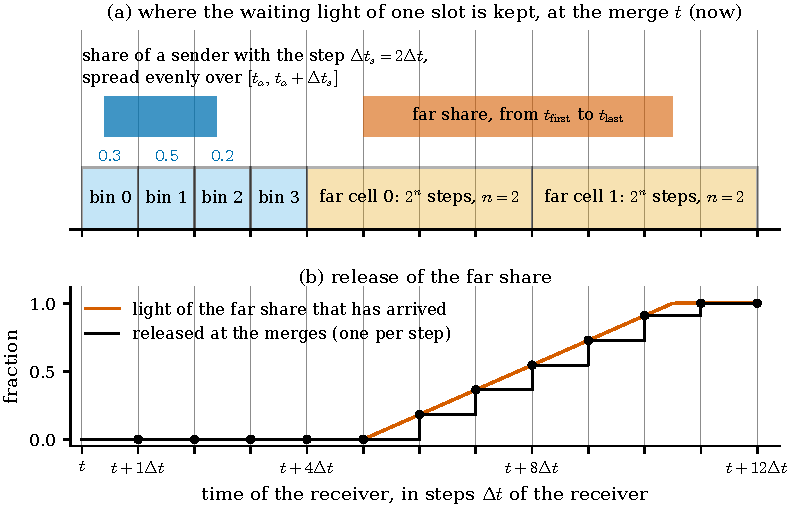
\includegraphics{figures/isrf_bins.pdf}
\caption{(a) The waiting light of one slot at a merge at time
$t$ (drawn with four near bins): $N_{\rm n}$ near bins one step wide, then two far cells $2^n$ steps wide ($n=3$
once the step is known; the drawing uses $n=2$). A share
from a sender with twice the step is spread over three bins.
(b) A far share is cut at the cell ends, and each piece leaves whole at the end
of its cell (black), never ahead of the arrived light (orange).}
\label{fig:isrf-bins}
\end{figure}

\subsubsection{Limit case: the no-delay test mode}
\label{sec:packet-reservoir}

In this mode, for tests, a share arrives at the next merge of its receiver
whatever the distance: the limit $v\to\infty$. It is the simple case of the
merge of Eq.~\eqref{eq:packet-merge-E}, with an inbox and a reservoir in place
of the near bins and far cells. A share goes into the inbox of the receiver slot, from which it joins the held
packet at the next active step of the receiver. This holds if the time bin of
the sender is not coarser than that of the receiver. If the bin of the sender
is coarser (its step is longer), the share goes into a reservoir of the slot
instead, with the same origin sum. The slot records the time $T_{\rm end}$:
the time of the booking plus one step of the current time bin of the source,
the latest over all shares of the slot. The reservoir is released in equal
parts over the step of the sender. At each merge of the receiver, at time $t$
and after a step of length $\Delta t$ (the step that ends now, which began at
$t-\Delta t$), the fraction
\begin{equation}
  f_{{\rm rel},k} = \begin{cases}
    \Delta t/(T_{\rm end}-t+\Delta t), & T_{\rm end}>t,\\
    1, & \text{otherwise}
  \end{cases}
  \label{eq:packet-release}
\end{equation}
of the reservoir joins the arrivals of the merge
(Eq.~\eqref{eq:packet-merge-E}). The fraction applies to the energy, the photon
number and the origin sum alike. Under cosmology $\Delta t$ and
$T_{\rm end}-t+\Delta t$ are proper times. With equal receiver steps the parts are equal: a share booked at
the start of a receiver step, with $n\Delta t$ to run, is released in $n$
merges of $1/n$ each, and the last merge releases the rest. If the part
released in a band, $f_{{\rm rel},k}$ times its photon number in the
reservoir, would be below $10^{-35}$, the whole reservoir is released, in every
band, with its origin sum. A star sends to the reservoir of a receiver whose
bin is finer than its own, with $T_{\rm end}$ the time of the emission plus
one step of its time bin.

\subsubsection{The field that the gas sees}
\label{sec:packet-field}

This step forms the moment $u_b$ of Eq.~\eqref{eq:isrf-moments}. The held
packet of a slot is the light that crosses the particle in one step over the
advance $l_{k}$ of Eq.~\eqref{eq:packet-advance}. Its flux through the volume
$m/\rho$ of the particle is $F=E_{k,b}\,\rho\,a\,l_k/(m\,\Delta t)$, and light of
that flux has the energy density $F/c$. The specific energy of band $b$ that
the particle sees is the sum over its slots,
\begin{equation}
  \tilde u_{b} = \sum_{k:\,S_k>0} \frac{E_{k,b}}{m}\,\frac{a\,l_k}{c\,\Delta t},
  \label{eq:packet-field}
\end{equation}
with $m$ the particle mass, $\Delta t$ the physical length of the step that
ends now and $c$ the speed of light; the photon number $N_{k,b}$ gives the
field of the photon number in the same way. The factor $a\,l_k/(c\Delta t)$ is
the hop speed over $c$ (Section~\ref{sec:packet-frame}). It is set to zero for
$\Delta t\le0$ or $m\le0$.

Why a sum of scalars gives the angular integral $c\,u_b=\oint I_b\,d\Omega$:
each slot holds the light of one range of directions, at most $90^\circ$ wide,
and its flux is computed with its own advance $l_k$. The speed at which that
slot's light moves cancels: in steady state a slower hop carries more energy
per step over a shorter advance, at the same flux. For light inside one cell,
$|\boldsymbol F_k|$ equals $\int_k I_b\,d\Omega$ up to the cosine spread of
the directions inside the cell, and the sum of $|\boldsymbol F_k|/c$ over the
slots is $u_b$.

The field can be averaged in time with an exponential running mean of time
constant $\tau_{\rm m}$ (default 0, i.e.\ off), which smooths light that
arrives in lumps,
\begin{equation}
  \bar u \leftarrow \bar u + (u-\bar u)\,\frac{\Delta t}{\tau_{\rm m}}, \qquad
  \bar u \leftarrow u \ \text{if}\ \tau_{\rm m}\le0\ \text{or}\ \Delta t\ge\tau_{\rm m}.
  \label{eq:packet-runmean}
\end{equation}
A step with $\Delta t\le0$ keeps the old mean. Only the field is averaged and
never the packet, so the ledger is not changed. Then, at the hop, each
particle $i$ takes the kernel mean of the fields of its neighbours and of
itself,
\begin{equation}
  \langle u_b\rangle_i =
  \frac{\sum_j m_j\,w(r_{ij}/h_i)\,\bar u_{b,j} + m_i\,w(0)\,\bar u_{b,i}}
       {\sum_j m_j\,w(r_{ij}/h_i) + m_i\,w(0)},
  \label{eq:packet-kernelmean}
\end{equation}
over the neighbours with $r_{ij}<\gamma h_i$, with $w(u)=h^3W(uh,h)$ the
kernel of the build without its factor $h^{-3}$. The kernel mean smooths the
particle-to-particle noise of the packet field. Its cost is resolution: it widens the edge of a shadow by up to
one kernel support radius $\gamma h_i$. The kernel mean $\langle u_b\rangle_i$
replaces the band values of the particle: PE, LW and the LW photon number. The
PE and LW energies give $G_0$ and $k_{\rm diss}$
(Eqs.~\eqref{eq:isrf-G0}, \eqref{eq:isrf-kdiss}). The LW photon number is an
output. The PE photon number is not kept.

\subsubsection{The frame of reference of the light}
\label{sec:packet-frame}

The packet transport works in the gas frame. Every offset is measured from the
particle that carries the packet. The stored origin of a slot is a distance and
a direction from its carrier (Section~\ref{sec:packet-merge}), and the offset
of a share is relative to its receiver (Eq.~\eqref{eq:packet-offset}). No
position in the box frame enters the light. The distance and the direction of
a held packet are set at the merge. The merge runs when the position of the
particle is updated (the drift), and the hop of the
same integer time reads them before the particle has moved, so they are never
stale. The offsets of the waiting light are different. They are measured
from the receiver at the time of booking, and stay as they are until the next
merge of the receiver, over any drift of the receiver in between. This is the
gas-frame choice.

The box frame is fixed in the comoving coordinates, in which the Hubble flow
is at rest; it differs from the gas frame by the peculiar velocities of the
gas. The choice of frame matters because a hop has the speed
$v_{\rm hop}=a\,l/\Delta t$, with $l$ the advance of
Eq.~\eqref{eq:packet-advance} and $\Delta t$ the step of the sender. This speed
is usually far below $c$ (Section~\ref{sec:isrf-speed}). In the box frame, a
source that moves with its gas at the bulk speed $V$ would leave its light
behind, by about $V/v_{\rm hop}$ hop lengths per hop. A uniform boost of the
whole box would then change the result. In the gas frame, only the velocity of
the source relative to the absorbing gas enters, and it is small for a star
that moves with its natal cloud. The Hubble flow is a coordinate effect that
comoving offsets absorb exactly.

The transport keeps the redshift of the Hubble flow and drops the terms of the
peculiar flow, the Doppler shift and the aberration. Per hop the dropped
Doppler term is of order $\Delta u/c$, with $\Delta u$ the relative velocity
of the sender and the receiver along the hop: $10^{-5}$ to $10^{-4}$ for
$\Delta u=3$ to $30\,{\rm km\,s^{-1}}$. The kept redshift over a $7$\,pc hop
is $\lambda\zeta$, with $\lambda$ the band-edge weight and
$\zeta=1.6\times10^{-9}$ at $z=0$ and $2.8\times10^{-8}$ at $z=9$
($H_0=70\,{\rm km\,s^{-1}\,Mpc^{-1}}$, $\Omega_{\rm m}=0.3$). Inside a galaxy
the dropped term per hop is therefore $10^{2}$ to $10^{3}$ times the kept one,
the ratio of the velocity gradient ($10\,{\rm km\,s^{-1}}$ over $100$\,pc,
$3\times10^{-15}\,{\rm s^{-1}}$) to $H$ ($2.3\times10^{-18}$ to
$3.9\times10^{-17}\,{\rm s^{-1}}$ from $z=0$ to 9).

Dropping the larger term is still the better choice, because the two terms
add up differently along a ray. The Doppler terms of successive hops along a
straight ray telescope: their sum is
$(\boldsymbol u_{\rm last}-\boldsymbol u_{\rm source})\cdot\boldsymbol n/c$, the
Doppler shift between the source and the last receiver, whatever the number of
hops. It stays of order $\sigma/c\approx10^{-4}$ for a velocity dispersion
$\sigma$ of a few tens of km\,s$^{-1}$. The Hubble term has one sign and grows
with the path, as $H\ell/c$. Inside a galaxy both are negligible against the
other errors of the scheme (Section~\ref{sec:isrf-accuracy}); in diffuse
intergalactic gas, where the peculiar gradient is of order $H$, the two are
comparable per hop. The aberration, of order $u/c$ in angle, is far smaller
than the width of a slot.

\subsubsection{How light merges}
\label{sec:packet-merge-summary}

Figure~\ref{fig:isrf-share} follows one share from the slot of its sender to
the held packet of its receiver. The unit of merging is the slot: light that
lands in two different slots of a particle is never merged. At the booking, a
share adds its energy, photon number and $e_s\boldsymbol{o}_s$ to a store of
the slot that its origin sets. At the next step of the receiver, the light
that is due leaves the stores and becomes the held packet
(Sections~\ref{sec:packet-merge} to \ref{sec:packet-reservoir}).
Table~\ref{tab:isrf-merge-rules} lists how each quantity is combined.

\begin{table}[htbp]
\centering
\caption{How the quantities of one slot are combined when light merges.}
\label{tab:isrf-merge-rules}
\small
\begin{tabular}{>{\raggedright\arraybackslash}p{4.4cm}>{\raggedright\arraybackslash}p{9.8cm}}
\toprule
quantity & rule \\
\midrule
energy $E_{k,b}$, photon number $N_{k,b}$ & summed, per band \\
origin of the packet & mean of the origin offsets, weighted by the energy of
  each share after redshift and dust, summed over both bands; one origin for
  both bands \\
direction $\boldsymbol{n}_k$, distance $d_k$ & taken from the mean origin
  (Eq.~\eqref{eq:packet-merge-origin}) \\
near bins (capped mode) & a bin that has ended is released whole \\
far cells (capped mode) & a cell is released whole at its end \\
origin sum (capped mode) & one sum for all waiting light; the fraction of the
  waiting energy that is released takes the same fraction of the sum \\
departure time (capped mode) & the merge time, kept as the end of the step minus the step \\
reservoir (no-delay mode) & the fraction $f_{{\rm rel},k}$ of its energy,
  photon number and origin sum joins the merge \\
\bottomrule
\end{tabular}
\end{table}

The mean is taken over origin offsets, not over unit directions: of two shares
of equal energy, the one with the more distant origin turns the merged
direction more.

\begin{figure}[htbp]
\centering
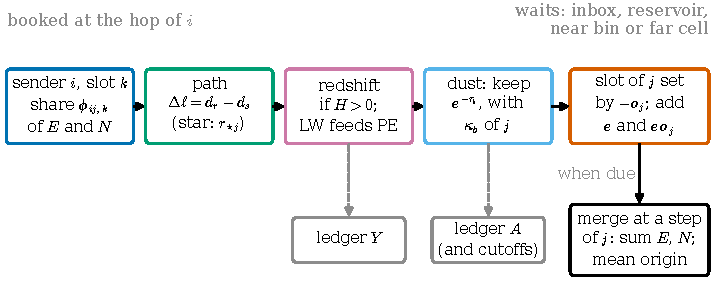
\includegraphics{figures/isrf_share.pdf}
\caption{The life of one share. It is booked at the hop of its sender:
first the path, then the redshift, then the dust, each with its ledger. It
then waits in the slot that its origin sets, and joins the held packet at a
merge of the receiver.}
\label{fig:isrf-share}
\end{figure}

\subsubsection{How light is absorbed}
\label{sec:packet-absorb-summary}

Dust acts once per share, when the share is booked: at the hop of the
sender, or at the emission of a star. The steps are, in order
(Fig.~\ref{fig:isrf-share}):
\begin{enumerate}
  \item The path. For a hop it is the increase of the distance from the
    origin of the packet, $\Delta\ell=d_r-d_s$; for a star it is the distance
    to the receiver (Eq.~\eqref{eq:packet-path}). The physical path is
    $a\,\Delta\ell$.
  \item The redshift, in an expanding box only
    (Section~\ref{sec:packet-transfer}). LW loses energy and photons, and part
    of them enters PE. The net loss goes to the redshift ledger $Y$.
  \item The dust. The receiver's $\kappa_b$ gives $\tau_b=\kappa_b a\Delta\ell$,
    and the share keeps $e^{-\tau_b}$ of its energy and of its photon number
    (Section~\ref{sec:packet-absorption}). The rest goes to the absorbed
    ledger $A$.
  \item What remains waits in the slot of the receiver. A band whose photon
    number would fall below $10^{-35}$ is booked whole into $A$, at the
    delivery or later at the release of a near bin or a far cell.
\end{enumerate}
The energy is therefore removed before the light waits for its arrival time.
The ledgers $A$ and $Y$ exist only in a diagnostic build; the removal is the
same without them.

The absorbed light does not heat the gas. The gas sees only the light that
crosses it, through $G_0$ and $k_{\rm diss}$ (Section~\ref{sec:packet-field}),
and Grackle applies no second dust attenuation to $G_0$. The transport has no
H$_2$ line absorption. When the H$_2$ self-shielding option of Grackle is on
(Section~\ref{sec:isrf-problem}), Grackle multiplies $k_{\rm diss}$ by a
factor \citep{WolcottGreenHaiman2019} from a local H$_2$ column: $n_{\rm H_2}$
times a multiple of the kernel support radius, or times the Jeans length.

% ---------------------------------------------------------------------------
\subsection{Numerics: speed, conservation, rounding, accuracy and limits}
\label{sec:isrf-numerics}

\subsubsection{The speed of the light and the time step}
\label{sec:isrf-speed}

The scheme moves the light by one hop per step of the sending particle. A hop
is the hand-over from a gas particle to its neighbours
(Section~\ref{sec:packet-hop}); its mean advance $l$ is a fraction of a
smoothing length. The speed of the light is therefore at most the hop speed
$a\,l/\Delta t$, with $\Delta t$ the step of the sender. In the capped and the
step-bounding modes it is also never faster than $v=fc$ in the frame of the
gas. The front thus moves at about $\min(v,\,a\,l/\Delta t)$. For an advance of
$1$\,pc and a step of $1$\,kyr this is $980$\,km\,s$^{-1}$, or
$3\times10^{-3}c$; Section~\ref{sec:isrf-accuracy} gives the measured value in
a test. The default capped mode and the no-delay mode set no bound on the time
step, so the light moves at the hop speed, far below $c$. The step-bounding
mode bounds the step of every gas particle by
\begin{equation}
  \Delta t \le f_{\Delta t}\,\frac{a\,h}{v},
  \label{eq:isrf-dt}
\end{equation}
with the margin $f_{\Delta t}$ (default 0.5), so that a hop is fast enough for
the light to move at $v$. Above $f_{\Delta t}$ of about 0.8 the bulk of the
light lags behind $v$, while its front, carried by the neighbours near the
kernel edge, keeps the speed. The bulk lags also below that value: in a beam
test with a step of $0.43\,h/v$ the centre of a light pulse moved at 0.64 to
$0.66\,v$ (Section~\ref{sec:isrf-accuracy}). The lag has two causes. A hop delays the light by its full length, but the
pulse gains only the part of the hop along its axis (a factor of about 0.83),
and a hop leaves at the end of a step of the receiver (a factor of about 0.78).
Together these give 0.645 at $0.43\,h/v$. A model built on these two factors
reproduces the speed measured at four step sizes to 0.013 of $v$. The bound costs many steps: at $v=0.99c$ and $h=0.2$\,pc it is $0.33$\,yr,
about $3\times10^4$ times shorter than the step of the test of
Section~\ref{sec:isrf-accuracy}. This mode is therefore affordable only with a
limit speed far below $c$.

A sender that moves towards the receiver between its merge and its booking, or
a receiver that speeds up after it, can make the front move at up to $v+u$ in
the frame of the box. This is harmless for $v$ near $c$. It is not for the slow
limit speeds that make the step-bounding mode affordable, when they approach
the speeds of the gas. A receiver that recedes
faster than $0.99\,v$ gets its light early (the cap on $v/(v-u_j)$ of
Section~\ref{sec:packet-lightspeed}). A diagnostic build counts these
deliveries.

\subsubsection{The reach of a hop}
\label{sec:isrf-reach}

The reach of a hop (Fig.~\ref{fig:isrf-hop}b) is the kernel support of the
sender, $r_{ij}<\gamma h_i$,
and, for a receiver $j$ that is active in this step, the kernel support of the
receiver, $r_{ij}<\gamma h_j$. Both radii are cut by the factor
$1-\delta_{\rm r}$. Without the cut, a pair at the edge could be inside
the reach when $S_{i,k}$ is summed and outside when the shares are booked,
because the two computations may round the distance differently.

The pair loops form $\boldsymbol{r}_{ij}$ in float from positions measured from
the corner of a cell. Along an axis the first position is at most $2W$ from
it and the second at most $W$, plus the drift since the last rebuild. The
rebuild criterion limits the sum of the two drifts to $W-R$, so
$|p_i|+|p_j|\le 4W-R$. The relative error of $r_{ij}^2$ at the edge $R=\gamma h$ is at most
$\sqrt{3}\,2^{-23}\,(|p_i|+|p_j|)/R$, plus the other roundings of the distance
(the difference, the sum of squares and the cut product). With
$|p_i|+|p_j|\le 4W$ the cut is
$\delta_{\rm r}=10^{-5}+2.1\times10^{-7}\cdot 4W/R$, at most $0.5$, with $W$
the largest top-level cell width, refreshed at every rebuild, and $R$ the edge
being tested. The bound needs a hydro pair task to limit the drift of a cell. A
gas cell whose 26 neighbours are all empty has no pair task, so no drift check
bounds it and the bound has no guarantee there; this is rare. The constant $10^{-5}$ is about a hundred float roundings of the
square distance and holds the other roundings. A wide cell, which holds a particle with a small
smoothing length in a cell sized for a larger one, gets a larger cut: for
$4W/R=100$ it is $3.1\times10^{-5}$. At startup rank 0 warns if the cut reaches its cap, and the verbose log gives
$W/R$ for the smallest smoothing length.

$S_{i,k}$ is summed in one pass over the neighbour pairs and the shares are
booked in a later pass, and a pair can be visited from either of its
particles. The weight uses the larger length $H_{ij}$, so that it has the same
value in both passes, from both sides and for an inactive receiver; the shares
of a sender then sum to one. The kernel mean of the field
(Eq.~\eqref{eq:packet-kernelmean}) moves no light and needs no such
agreement. It uses the support $\gamma h_i$ of the particle alone, the usual
SPH gather; this is a choice. A pass visits a pair only for an active
particle, and only inside its kernel support. A neighbour $j$ with
$\gamma h_i\le r_{ij}<\gamma h_j$ is therefore seen only when $j$ is visited,
which needs $j$ active: an inactive receiver beyond $\gamma h_i$ gets no
light. The booking pass books each part in the same visit as the summing pass
adds it: the inner part in the visit of the sender, the outer part in the
visit of the receiver, because the visit of the sender at its own tree depth
need not reach a receiver with a larger smoothing length. The reach is a geometric bound, not a light travel distance. The speed
of light limits when a share arrives, not how far it reaches.

\subsubsection{Absorption over a hop}
\label{sec:isrf-hop-absorption}

A share is absorbed with the $\kappa_b$ of its receiver over its whole path
(Eq.~\eqref{eq:packet-tau}), so $\kappa_b$ is constant along each hop. Between
gas of different density the optical depth of a hop is that of the receiver,
not the integral along the segment. The edge of a shadow can therefore sit up
to one hop downstream of the edge of the absorbing gas.

\subsubsection{Conservation and the ledgers}
\label{sec:packet-ledger}

The light is accounted for per band, in energy and in photon number
($N E_{\rm lo}$). The ledgers exist only in a diagnostic build. Without them
the transport is the same, but nothing books the amounts below. Every gas particle carries three
cumulative ledgers:
\begin{itemize}
  \item the absorbed ledger $A$ (Section~\ref{sec:packet-absorption}); it
    also holds the light dropped below the photon cutoff of $10^{-35}$, at
    the delivery and at the release of a near bin or a far cell;
  \item the redshift ledger $Y$ (Section~\ref{sec:packet-transfer}; zero in a
    static box);
  \item the escaped ledger $X$: the held light of a slot with no downstream
    neighbour (Section~\ref{sec:packet-hop}) is added to $X$ and set to zero.
\end{itemize}
Every star carries the energy emitted, $E_{\rm em}=L_b\Delta t_\star$ summed
over its steps, and the energy escaped,
$X_\star=L_b\Delta t_\star\sum_c\varepsilon_c$ (Eq.~\eqref{eq:packet-escape}),
together with the photon numbers $f_b$ times these. A gas particle can become
a star, be swallowed by a sink, or become a sink. The light it still holds in
flight is then lost with it. This is, in all slots, the held packet and the
waiting light in all its stores. It is booked as removed energy $E_{\rm rm}$ in the ledger
of the star or the sink. The absorbed, the redshift and the escaped ledgers of
the gas are carried over in the same ledger as inherited amounts
$E_{\rm inh}$. When a sink
swallows another, the survivor adds the ledger of the swallowed sink to its
own. Gas that leaves a non-periodic box is booked in the same way, into a
box ledger. A star or a sink that leaves such a box is booked into the box
ledger with its own ledger, and so is the gas that a black hole swallows. The
box ledger is summed over the ranks and written with each snapshot. With
$E_{\rm fl}$ the light in flight, the amounts of one band balance as
\begin{equation}
  \sum_{\star,\,{\rm box}} E_{\rm em} =
  \sum_{\rm gas}\big(A+X+Y+E_{\rm fl}\big) + \sum_{\star,\,{\rm sinks},\,{\rm box}}\big(X_\star + E_{\rm rm} + E_{\rm inh}\big),
  \label{eq:packet-balance}
\end{equation}
where ``box'' marks the entries of the box ledger: the stars that left the box
add their emitted energy to the left side, and the stars, the sinks, the gas
that left the box and the gas swallowed by black holes add their ledgers to
the right side. Likewise for the photon number. In each band, $Y$ is booked net of the gain
from the other band, so $Y_{\rm PE}$ can be negative, and the balance of each
band is exact.

Each step of the transport moves light between the terms without creating or
destroying it. The hop shares sum to one (Eq.~\eqref{eq:packet-share}); the
merge adds; the redshift moves the lost part to $Y$; the absorption moves the
absorbed part to $A$. The cell fractions of a star sum to one only if the
pass that sums $S_c$ and the later pass that delivers the shares see the same
receivers and the same $h_\star$. The balance holds up to the rounding of float
arithmetic; in the beam tests of Section~\ref{sec:isrf-accuracy} the energy of
the light is kept to $2\times10^{-7}$ of the beam energy or better. The term
``left'' of Eq.~\eqref{eq:packet-balance} is the ledger of the gas that left a
non-periodic box ($X_\star=0$ there). Test beams, light placed directly into
the gas at the start of a run without a star, are in no ledger and are not part
of Eq.~\eqref{eq:packet-balance}.

\subsubsection{Rounding}
\label{sec:isrf-rounding}

The ledgers are in double precision, because small shares must not be lost
against a large total. A stored share is a float, with a relative rounding of
at most $2^{-24}$, about $6\times10^{-8}$. The relative loss of a share in one
hop by the redshift is $\lambda\zeta$, with $\lambda$ the band-edge weight. For
a $7$\,pc hop with the default weights it is about $10^{-8}$ in LW at $z=0$,
and $1.8\times10^{-7}$ in LW and $6\times10^{-8}$ in PE at $z=9$. Below $z$ of
about 4 the LW loss of one hop is below the rounding, so the stored shares
carry it only on average. At higher redshift they resolve it. The double
ledger $Y$ books it in both cases.

\paragraph{Stochastic rounding of the sums.} A float running sum rounded to the
nearest drops every term below half a step of the sum. The hop weights and
the shares have a long tail of such terms. The weight sum $S_{i,k}$ and the
inbox of a slot would then come out low, and a fixed fraction of the light in
flight would be lost or created at each step. The scheme therefore adds these
terms with stochastic rounding. The exact sum is formed in double precision and
rounded to the float below or above it, with the probabilities that make the
result exact on average. The random bits are a hash of the two operands and of
a salt that changes from one addition to the next (the receiver, the share and
the step). The hash keeps no state. A sum that a float holds exactly is
returned exactly.

\paragraph{Order of the additions.} Shares reach a slot from many senders, in
an order set by the scheduling of the tasks on the threads. Float addition is
not associative, and the rounding of each addition depends on its operands.
Two runs with the same input can therefore differ in the last bits of a slot,
and the difference is then carried along the transport. This noise is unbiased: it
does not change the balance of Eq.~\eqref{eq:packet-balance} beyond the
rounding of each addition. At the default speed it stays small: in a beam
test two runs on four threads differ by $6\times10^{-6}$ of the beam energy
(Section~\ref{sec:isrf-accuracy}). At a slow limit speed in the step-bounding
mode the difference grows, from $10^{-6}$ to $4\times10^{-2}$ over the same
test, by a mechanism not yet identified; one-thread runs are bit-identical.

\subsubsection{Measured accuracy}
\label{sec:isrf-accuracy}

Three tests measure the accuracy of the transport: one star in uniform gas, the
sideways spread of a beam, and two crossing beams. Each was run with 12
slots, $p=4$ and at one resolution unless stated.

\paragraph{One star: the thin limit and a shadow.} Figure~\ref{fig:isrf-thin}
shows one star in a static box, $10$\,pc wide and not periodic, in the default
capped mode at $0.99\,c$. The box holds uniform gas of
$n_{\rm H}\approx720$\,cm$^{-3}$ and metallicity $Z=2\times10^{-4}$ in
$262\,144$ particles, so $\tau_{\rm PE}=0.03$ per pc. The steps of the gas are
at most $9.2$\,kyr. Panel (a) plots $c\rho\tilde u_{\rm PE}$, the median in
shells around the star. Inside the front it is 0.90 to 0.95 times
$L_{\rm PE}e^{-\kappa_{\rm PE}r}/(4\pi r^2)$; the cause of the deficit of 5 to
10 per cent is not known. The front reaches about $2.5$\,pc at $0.15$\,Myr and
$5$\,pc at $0.29$\,Myr. It moves by $0.16$\,pc, one particle spacing, in each
step of $9.2$\,kyr: $17$\,km\,s$^{-1}$ or $6\times10^{-5}c$. Real light
crosses $2.8$\,kpc in one such step, and $90$\,kpc in $0.29$\,Myr. Behind the front the field is close to the
steady field; ahead of it the gas sees none of the light. In this test a new
star lights the gas at $5$\,pc after $0.29$\,Myr, not after $16$\,yr.
Panel (b) adds a clump of radius $1$\,pc on the line of sight, at the same
density and $165$ times the metallicity, so that $\tau_{\rm PE}=10$ through its
centre. The ratio of the fields with and without the clump, the median in a
thin cylinder around the axis, follows $e^{-\kappa_{\rm c}\ell}$ over four
decades, with $\kappa_{\rm c}$ the absorption rate of the clump and $\ell$ the
depth into it.

\begin{figure}[htbp]
\centering
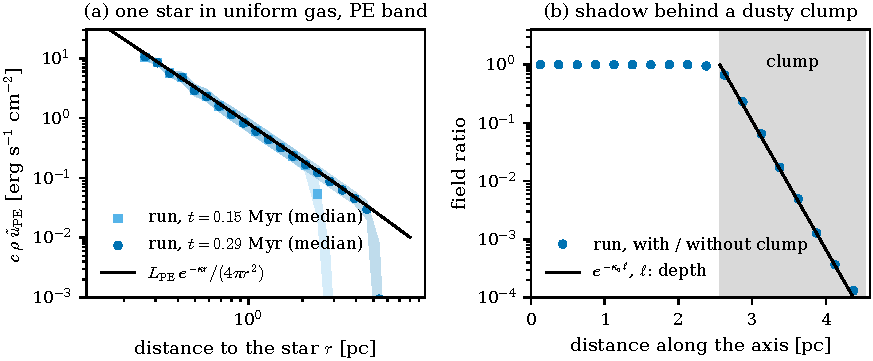
\includegraphics{figures/isrf_thin.pdf}
\caption{One star in a run of the scheme. (a) The field that Grackle
receives, at two times, against the thin limit of Eq.~\eqref{eq:isrf-thin}.
Inside the front they agree to 10 per cent; the front is far slower than
light. (b) The field with a dusty clump over the field without it falls as
$e^{-\kappa_{\rm c}\ell}$: a sharp shadow.}
\label{fig:isrf-thin}
\end{figure}

\paragraph{Sideways spread of a beam.} The hop cone spreads a beam sideways.
The spread was measured in a periodic glass of $98\,304$ particles without
absorption, on a cube of light, $10\,h$ wide, that moves along one axis with
its origin far behind (a collimated beam). The variance of the light across
the beam, per axis, grows linearly with the distance $s$ travelled:
$\sigma^2-\sigma_0^2=A\,s$. The spread is diffusive: the width grows as
$\sqrt s$, not in proportion to $s$. The coefficient is $A=0.261\,h$,
$0.168\,h$ and $0.116\,h$ for $p=2$, 4 and 8. After $100\,h$ the rms
sideways shift per axis is $5.1$, $4.1$ and $3.4\,h$. A larger $p$ narrows
the beam at no memory cost; its other costs are not measured, and at $p=8$ the
spread already follows the structure of the glass more. Two orientations of the
slot frame, with the beam $10.7^\circ$ and $29.1^\circ$ from a slot border,
give the same $A$ to four digits. A test beam whose origin lies one smoothing
length behind each particle instead fans out like many point sources, with a
spread angle of $12.6^\circ$; at $27\,h$ its variance is seven times that of
the collimated beam. This spread comes from the setup of such a beam, not from
the hop.

\paragraph{Crossing beams.} Free streaming is linear, so two beams that cross
must give the sum of the two single-beam fields. The test measures the
summed absolute difference between the two, over the summed energy; exact
transport gives 0. Two pulses crossed head-on in a glass of $884\,736$
particles without absorption. In the default capped mode the difference after
the crossing is at most $5.1\times10^{-5}$ (fan beams, $d=1$), three to nine times the
difference between two identical runs. In the step-bounding mode at
$v=3\times10^{-5}c$ ($9$\,km\,s$^{-1}$), with one thread, it is
$2.0\times10^{-2}$ to $3.1\times10^{-2}$. At a slow limit speed the transport
is therefore not linear even for opposite beams; the mechanism is not known. In
that run, with a step of $0.43\,h/v$, the centre of a pulse moves at
$0.64\,v$, and at $0.66\,v$ with eight times more particles. Beams at
$60^\circ$ share slots; that limit follows.

\paragraph{What is not established.} No accuracy test of the transport ran in
an expanding box: the redshift and the band-edge transfer have only the
per-hop error sizes of Sections~\ref{sec:packet-transfer} and
\ref{sec:isrf-rounding}, and the cosmological equation has no end-to-end test.
The accuracy on several MPI ranks is not measured. There is no resolution
study, no study of the slot count $K$, no comparison with an independent
transfer code other than on beam tests, and no galaxy-scale test.

\subsubsection{Limit: merged slots break the linearity of the superposition}
\label{sec:packet-superposition}

The transport is linear in the energy that each source emits, as long as every
source keeps its own slots. It is not exactly linear when two sources send
light into the same slot of a receiver. The slot then keeps one mean origin and
one direction (Eq.~\eqref{eq:packet-merge-origin}), and the later hops use that
merged direction. The field of two sources is then not the sum of the fields
that each source gives alone. Two cases fall under this limit:
\begin{itemize}
  \item two beams or stars whose light reaches a gas particle from directions
    less than about one slot apart;
  \item the spread of the transmission cone, which carries a part of a beam
    into the neighbouring slots.
\end{itemize}
The size of the effect was measured with 12 slots in a gas box crossed by two
fan test beams (origin distance $d=1$). For two fan beams at $60^\circ$
(Fig.~\ref{fig:isrf-merge}b), $87.6\,\%$ of the light of the first beam
arrives in one slot of the receivers, and $8.4\,\%$ of the light of the second
beam arrives in the same slot. After 24 steps of the two beams together, the
field differs from the sum of the fields of the two single-beam runs by a
fraction $5.4\times10^{-2}$. With the collimated default ($d=1000$) the same
crossing gives $2.2\times10^{-8}$ after 20 steps, where the fan gives
$9.7\times10^{-2}$ in the same setup: a collimated beam keeps to its own slots.
Two collimated beams $30^\circ$ apart, which fall in one slot, still give
$1.07$, so the limit remains. For fan beams at $180^\circ$ the fraction is
$3.7\times10^{-6}$, close to the rounding of the single precision sums,
because the beams then use opposite slots. Opposite beams are not always
additive: the crossing test of Section~\ref{sec:isrf-accuracy} gives up to
$5.1\times10^{-5}$ at the default speed and $2\times10^{-2}$ at a slow limit
speed. For two stars in a
low-resolution box, the total light summed over all gas particles after 64
steps differs from the sum of the two single-star runs by a fraction
$1.3\times10^{-4}$. The light of a single gas particle, and so its $G_0$, can
differ by up to $13\,\%$. The scheme conserves the energy of each band exactly
in every case (Section~\ref{sec:packet-merge}); what it loses is the exact
additivity of the directions.

The scheme has no correction for this: it keeps the total energy, but not the
field of several sources at a single particle.

\subsubsection{Limit: the far light at a slow speed}
\label{sec:isrf-far-limit}

A far cell keeps one time for all its light and leaves whole at its end, so
light that arrives beyond the $N_{\rm n}$ near bins leaves in lumps. Take one
receiver fed by one steady sender. A merge releases at most the light that
arrived within one cell width $W$ steps, which is $W$ times the mean per
merge. The largest $|{\rm held}-{\rm mean}|/{\rm mean}$ is therefore 0 while
all the light of the sender arrives within $N_{\rm n}$ receiver steps of the booking,
and at most $W-1$ beyond, with $W=8$ as long as no light is beyond the last
cell of $8$ steps. A sender farther than that cell widens the cells to $W>8$
steps, and the bound is then $W-1$ with the widened $W$. It grows with the part
of the light beyond the $N_{\rm n}$ near bins: for $N_{\rm n}=4$, a sender 2 or 4 times coarser than the receiver gives 0 when its
whole window lies in the near bins, between 0.15 and 6.1 when part of it does
not, and 7 at a delay of 10 receiver steps. The mean over a window of $n$ merges is
off by at most one cell content, $W/n$ of the mean. It does not occur at the
default $v=0.99c$, nor in the step-bounding mode with $f_{\Delta t}=0.5$,
except for the outermost neighbours: a hop to the kernel edge is 3.9 receiver
steps, up to 7.7 with the bin rounding, so with $N_{\rm n}=4$ their light
leaves in lumps of up to $W-1$. With the default 8 bins the demand
$\lceil 1.94/f_{\Delta t}\rceil+s$ is 8 at $s=4$ and $f_{\Delta t}=0.5$, so
it fits for a sender up to 4 times coarser than the receiver, and lumps only
for a coarser sender, which the time-step limiter does not allow at the choice
of a step but can occur after a drop of the receiver step.

% ---------------------------------------------------------------------------
\subsection{Comparison with TRAPHIC}
\label{sec:isrf-traphic}

TRAPHIC, the transport of photons in cones, is the published method closest
to this scheme \citep{PawlikSchaye2008,PawlikSchaye2011}. It transports
hydrogen- and helium-ionising radiation in SPH simulations of reionisation.
This subsection compares the two as those papers describe TRAPHIC.
Table~\ref{tab:isrf-traphic} sets them side by side.

\paragraph{What the two share.} Both move the light from SPH particle to
neighbour, with no grid: random emission cones at a source, transmission only
to the neighbours ahead, and reception cones whose packets merge into one. The
cost does not grow with the number of sources. Both absorb $1-e^{-\tau}$ over
a hop with the density of the receiver, and in both a merge replaces the
directions by a mean, so several sources do not add exactly.

\begin{table}[!htbp]
\centering
\caption{TRAPHIC, as described by \citet{PawlikSchaye2008,PawlikSchaye2011},
and the packet transport of this channel.}
\label{tab:isrf-traphic}
\footnotesize
\begin{tabular}{>{\raggedright\arraybackslash}p{2.3cm}>{\raggedright\arraybackslash}p{5.9cm}>{\raggedright\arraybackslash}p{5.9cm}}
\toprule
aspect & TRAPHIC & this scheme \\
\midrule
radiation & ionising photons; one frequency (2008), several frequency bins
  for H and He with photoheating (2011) & non-ionising: two bands, PE and LW;
  energy and photon number per band \\
a packet holds & photon number of one frequency, a direction, a clock & energy
  and photon number of both bands, one direction, the distance to its origin;
  an arrival time under a speed limit \\
emission & $N_c$ cones of equal solid angle, random rotation at each emission;
  equal weight per neighbour in a cone, the light of a cone by its solid
  angle; a virtual particle in an empty cone & 12 HEALPix cells, random
  rotation per star and step; volume and tent weight, one share law over all
  cells; a cell with too little gas lets its part escape \\
transmission & neighbours inside a regular cone of solid angle $4\pi/N_c$
  around the direction, equal weights; a virtual particle if the cone is empty
  & every neighbour ahead ($\mu>10^{-3}$), weight $V_jW\mu^p$, $p=4$; the
  light escapes if there is none \\
reception & $N_c$ cones, random rotation at each reception; a packet is binned
  by its direction & $K=12$ cells (8, 16, 24 or 48), one fixed frame for all particles
  and steps; a share is binned by the direction from its origin to the
  receiver \\
merging & mean of the unit directions, weighted by the photon number and
  normalised; mean of the clocks; each frequency apart & mean of the origin
  offsets, weighted by the energy of both bands; direction and distance
  from it; latest arrival time \\
absorption path & projection of the hop on the direction; the full distance
  from a source & increase of the distance from the origin; the full distance
  from a star \\
use of the absorbed light & the absorbed photons give the photoionisation
  rate; ionisation and temperature are sub-cycled & a sink only, in a ledger;
  the gas sees the light that crosses it, through $G_0$ \\
speed of light & clock advanced by $d/c$ per hop, packet held until the
  simulation time reaches it; or the time-independent limit, one particle
  spacing per step & arrival time at $v=0.99\,c$, at most one hop per step of
  the sender; a step-bounding mode so the front moves at $v$, and a
  no-delay mode for tests \\
time steps & one global radiative transfer step $\Delta t_{\rm r}$ & the
  individual time bins of the gas; near bins and far cells \\
cosmology & tested on a static density field at $z\approx8.85$; the clock is
  noted as a way to redshift & comoving offsets; redshift and band-edge
  transfer per share \\
cost & $\propto N\tilde N_{\rm ngb}N_c$ with the box full of light; at most
  $N_c$ packets per frequency per particle & $\propto$ active gas $\times$
  neighbours $\times K$ per step; $K$ slots per gas particle \\
resolution & $\tilde N_{\rm ngb}$ (32 in the tests) and $N_c$ (8 to 128;
  32 converged in the reionisation test) & the hydro neighbours, $K$ and $p$ \\
known artefacts & particle noise, largest at $N_c=\tilde N_{\rm ngb}$ and
  reduced by resampling; shadows slightly wider for
  $N_c>\tilde N_{\rm ngb}$; overshoot of less than one hop per step; merged
  clocks change the distance travelled & merged
  slots break linearity; thread-order rounding noise; lumps of far light at
  slow speeds; shadow edge up to one hop late; front slower than $v$ \\
\bottomrule
\end{tabular}
\end{table}

\paragraph{Merging.} This is the main difference. TRAPHIC keeps a direction
and a clock per packet and does not carry the position of the source. It
merges the directions of a reception cone as a mean of unit vectors, weighted
by the photon number and normalised \citep[Section~4.2.3]{PawlikSchaye2008}
\citep[footnote~6]{PawlikSchaye2011}. This scheme keeps the distance to the origin
as well. It merges the origin offsets, weighted by the energy, and takes the
direction and the distance from the mean origin
(Section~\ref{sec:packet-merge-summary}). The distance sets the absorption
path of the next hop, and the slot of each receiver. TRAPHIC bins a packet by
its own direction; this scheme bins a share by the direction from its origin
to the receiver, so the light keeps a straight line away from its origin.
TRAPHIC rotates its reception cones at random at each reception. This scheme
uses one fixed frame, so a beam along a cell border can fall on either side
(Section~\ref{sec:packet-state}).

\paragraph{Cones and empty cones.} TRAPHIC sends to the neighbours inside a
regular cone. Its opening angle $\omega$ follows from
$\Omega_t=4\pi/N_c=2\pi(1-\cos\omega/2)$, about $41^\circ$ at $N_c=32$. This
scheme weights every neighbour ahead by $\mu^4$, which falls to one half at
$33^\circ$ from the direction. A regular cone with the solid angle of one of
12 slots has $\omega=67^\circ$, a half-angle of $34^\circ$: the two widths
are close. Where a cone holds no neighbour, TRAPHIC creates a virtual particle
and loses no light. This scheme books that light as escaped, at the emission
(Eq.~\eqref{eq:packet-escape}) and at a hop (Section~\ref{sec:packet-ledger}).

\paragraph{Absorption and its use.} For a hop TRAPHIC takes the projection of
the separation on the direction. The increase of the distance from the origin,
used here, equals it when the origin is far compared with the hop. In TRAPHIC
the absorbed photons give the photoionisation rate of the receiver, and
photons that the sub-cycled rate equation does not use return to the
transport \citep[Section~5.2]{PawlikSchaye2008}. Here the absorbed energy is a
diagnostic; the gas responds to the light that crosses it.

% ---------------------------------------------------------------------------
\subsection{In the code}
\label{sec:isrf-code}

All locations are relative to the repository root. Line numbers refer to the
source files at the code version that this document describes; where lines
move, find the construct by name. The
transport needs the HEALPix C library (\code{--with-chealpix}).

\paragraph{Coupling to Grackle (Sec.~\ref{sec:isrf-problem}).} $G_0$,
Eq.~\eqref{eq:isrf-G0}, is \code{radiation\_get\_part\_isrf\_habing}
(\code{src/feedback/GEAR/radiation\_gas.c:768-787}), and $k_{\rm diss}$,
Eq.~\eqref{eq:isrf-kdiss}, is
\code{radiation\_get\_part\_LW\_dissociation\_rate\_internal} (:805-826). Each
band is clamped to zero by \code{radiation\_get\_band\_u\_nonnegative}
(:741-751). The constants $F_{\rm H}$ and $\sigma_{\rm H_2}/\bar E_{\rm LW}$ are
\code{RADIATION\_HABING\_FLUX\_CGS} and
\code{RADIATION\_SIGMA\_H2\_OVER\_E\_LW\_CGS}
(\code{src/feedback/GEAR/radiation.h:81}, :88). Grackle reads the two rates
through \code{cooling\_get\_isrf\_habing\_subgrid} and
\code{cooling\_get\_LW\_dissociation\_rate\_subgrid}
(\code{src/cooling/grackle/cooling\_gear\_subgrid.h:267-299}). The second
returns zero for the build modes \code{grackle\_0} and \code{grackle\_1}
(\code{COOLING\_GRACKLE\_MODE} below 2, set by \code{--with-cooling}), whose
chemical network has no H$_2$. Both are called in
\code{cooling\_copy\_to\_grackle} (\code{src/cooling/grackle/cooling.c:903-939}). \code{dust\_chemistry},
\code{photoelectric\_heating} and \code{use\_isrf\_field} are switched on at
\code{cooling.c:1851-1855}. The H$_2$ self-shielding option of
Sec.~\ref{sec:packet-absorb-summary} is \code{GrackleCooling:H2\_self\_shielding}
(\code{src/cooling/grackle/cooling\_io.h:391-405}). Its values, not to be
confused with the build modes, are 0 (off, the default), 2 (the kernel-support
length) and 3 (the Jeans length). The length for the value 2 is set at
\code{cooling.c:945-952}. The option is read in every
build mode, but it acts on $k_{\rm diss}$, which is zero below
\code{grackle\_2}, so it has an effect only in \code{grackle\_2} and
\code{grackle\_3}. The LW photon
number is output only
(\code{src/feedback/GEAR\_thermal/feedback\_io.h:346-351}).

\paragraph{The light of a star (Sec.~\ref{sec:isrf-problem}).} A single star
sets $L_{\rm PE}$, $L_{\rm LW}$ and its photon fractions in
\code{stellar\_evolution\_compute\_preSN\_feedback\_individual\_star}
(\code{src/feedback/GEAR/stellar\_evolution.c:1393-1415}), from the table
datasets \code{L\_PE}, \code{L\_LW}, \code{MeanPhotonEnergyPE} and
\code{MeanPhotonEnergyLW}. A population does it in
\code{stellar\_evolution\_compute\_preSN\_feedback\_spart} (:1662-1706), from
\code{Integrated\_L\_PE}, \code{Integrated\_L\_LW} and the
\code{Integrated\_MeanPhotonEnergy*} datasets, up to the mass
\code{m\_sup\_capped} (:1635 for a table with a metallicity axis). The tables
are read in \code{src/feedback/GEAR/radiation\_table\_io.c} (:990, :1012,
:1112, :1138).

\paragraph{Without transport (Sec.~\ref{sec:isrf-problem}).} The local
deposit with $e^{-\kappa_b\ell}$ is in \code{radiation\_iact.h}
(\code{src/feedback/GEAR/radiation\_iact.h:279-323}), with the path
\code{radiation\_get\_comoving\_extinction\_path} and the factors
\code{radiation\_get\_part\_ISRF\_extinction\_factors}
(\code{src/feedback/GEAR/radiation\_isrf.c:265-309}, :434-454). The switch
\code{GEARFeedback:ISRF\_propagation} (0 off, 1 the transport) is parsed at
\code{src/feedback/GEAR\_thermal/feedback\_properties.h:827-828}, and the
choice of the length $\ell$, \code{GEARFeedback:ISRF\_extinction\_path}, at
:784.

\paragraph{Dust absorption rate (Sec.~\ref{sec:isrf-rte-static}).}
Eq.~\eqref{eq:isrf-kappa} is \code{radiation\_get\_part\_linear\_absorption\_rate}
(\code{radiation\_isrf.c:408-417}), through
\code{radiation\_get\_dust\_mass\_opacity} (:358-369) and
\code{radiation\_get\_dust\_to\_gas\_ratio\_relative\_to\_MW} (:337-344). The
constants are at \code{radiation.h:65-78}.

\paragraph{Band-edge weights (Sec.~\ref{sec:isrf-rte-comoving}).}
$\lambda_E({\rm PE})$, $\lambda_E({\rm LW})$ and $\lambda_N({\rm LW})$ are
computed from the integrated table by
\code{radiation\_set\_band\_edge\_coefficients}
(\code{src/feedback/GEAR/radiation.c:57-195}). They fall back to \code{RADIATION\_BAND\_EDGE\_WEIGHT\_PE\_DEFAULT} (2.154),
\code{RADIATION\_BAND\_EDGE\_WEIGHT\_LW\_DEFAULT} (6.508) and
\code{RADIATION\_BAND\_EDGE\_PHOTON\_WEIGHT\_LW\_DEFAULT} (6.0)
(\code{radiation.h:136-138}) when radiation is inactive or a luminosity
vanishes. They are stored as \code{band\_edge\_weight\_pe},
\code{band\_edge\_weight\_lw} and \code{band\_edge\_photon\_weight\_lw}
(\code{src/feedback/GEAR\_thermal/feedback\_properties.h:181-183}).

\paragraph{The packet and its slots (Sec.~\ref{sec:packet-state}).} The slot
count is \code{RADIATION\_PACKET\_SLOTS}, set by
\code{--with-isrf-packet-slots=<N>} (\code{configure.ac:3048-3056}, default 12;
\code{N} other than 8, 12, 16, 24 or 48 is an error; the default and the check are
repeated at \code{src/feedback/GEAR\_thermal/feedback\_struct.h:140-190}). The
slot struct is \code{feedback\_isrf\_packet\_slot\_data}
(\code{feedback\_struct.h:344-404}); the packet is
\code{feedback\_isrf\_packet\_data} (\code{feedback\_struct.h:410-440}).
Eq.~\eqref{eq:packet-meanE} is the definition in the comment of
\code{feedback\_isrf\_packet\_band\_data} (\code{feedback\_struct.h:251-258}).
Eq.~\eqref{eq:packet-photonfrac} is
\code{radiation\_set\_star\_packet\_photon\_fraction}
(\code{src/feedback/GEAR/radiation.h:385-396}, the ratio at :395). The
transport stops at start-up if a yields table lacks \code{MeanPhotonEnergyPE}
or \code{Integrated\_MeanPhotonEnergyPE}
(\code{src/feedback/GEAR\_thermal/feedback\_properties.h:913-921}).
Eq.~\eqref{eq:packet-slot8} is \code{radiation\_packet\_octant}
(\code{src/feedback/GEAR/radiation\_packet.c:808-819}), and
Eqs.~\eqref{eq:packet-slot8}--\eqref{eq:packet-slot48} are
\code{radiation\_packet\_slot} (\code{radiation\_packet.c:847-888}).
Eq.~\eqref{eq:packet-frame} is \code{radiation\_packet\_build\_octant\_frame}
(\code{radiation\_packet.c:942-998}). Its angles are
\code{GEARFeedback:ISRF\_packet\_octant\_frame\_angles\_deg} and its seed offset
\code{GEARFeedback:ISRF\_packet\_octant\_frame\_seed\_offset}
(\code{feedback\_properties.h:864-868}). The frame and the cone power are run
constants: \code{radiation\_packet\_set\_frame} (\code{radiation\_packet.c:278-282})
copies them into the globals \code{radiation\_packet\_octant\_frame} and
\code{radiation\_packet\_cone\_power}, at start-up and after a restart
(\code{radiation\_packet\_startup}, :571-572).

\paragraph{24 and 48 slots and their cost (Sec.~\ref{sec:packet-state}).}
\code{--with-isrf-packet-slots=24} and \code{=48} select two more partitions
(\code{radiation\_packet.c:864-878}). Let $m$ be the axis of the largest $|y|$
(the lowest axis on a tie), $s=[\,y_m\ge0\,]$, $(m_1,m_2)$ the two other axes
in axis order, $t=[\,|y_{m_1}|\ge|y_{m_2}|\,]$, and $b$ and $c$ equal to
$[\,y\ge0\,]$ for the larger and for the smaller of $|y_{m_1}|$ and
$|y_{m_2}|$. Then $k=4(2m+s)+2t+b$ for $K=24$, the faces of a tetrakis
hexahedron (each face of the cube cut by its two diagonals), and
$k=8(2m+s)+4t+2b+c$ for $K=48$, the faces of a disdyakis dodecahedron (those
triangles halved again). Both are convex spherical triangles of solid angle
$4\pi/K$, the opposite direction lies in another cell, and a tie goes to the
same side whatever the sign of a zero. The default frame keeps the box axes
$5.98^\circ$ from a border for both, against $10.54^\circ$ for $K=12$. The
border distance of the debug check is
\code{radiation\_packet\_slot\_border\_distance} (\code{radiation\_packet.c:903-929}).
\code{tests/testRadiationPacketSlotGeometry.c} checks these properties for the
slot count of the build against the nearest of $K$ generator directions.
Every gas particle holds the $K$ slots (\code{feedback\_struct.h:416}), so
its size grows by 272 bytes per slot (paragraph on memory below). The gradient and the force loops visit
every non-empty slot of the sender (\code{radiation\_packet.h:403}, :646), so
the work of a hop grows with the number of lit slots, at most $K$. More slots
narrow the limit of Sec.~\ref{sec:packet-superposition}: two directions share a
slot only if they are at most the largest angle inside a cell apart, $90^\circ$
for $K=12$, $\arccos(1/3)=70.53^\circ$ for $K=24$ (two cube vertices of a cell)
and $\arccos(1/\sqrt3)=54.74^\circ$ for $K=48$ (face centre and cube vertex).
The energy of each band is exact at every $K$.

\paragraph{The hop (Sec.~\ref{sec:packet-hop}).} The weight of
Eq.~\eqref{eq:packet-share} is \code{radiation\_packet\_transmission\_weight}
(\code{radiation\_packet.c:740-757}). It is out of line and divides $m_j$ by
$\rho_j$ inside, so the gradient loop and the force loop use the same compiled
arithmetic. Both loops give it the vector from
\code{radiation\_packet\_weight\_vector} (\code{radiation\_packet.c:776-790}),
computed once from the absolute positions in double, so the two loops agree on
the weight of every pair they both visit; the loop's own vector only selects the periodic image. The cutoff $\mu_{\rm min}$ is \code{RADIATION\_PACKET\_MU\_MIN}
(\code{src/feedback/GEAR/radiation\_packet.h:53}). The coefficients of
Eq.~\eqref{eq:packet-kernel} are \code{kernel\_coeffs}, \code{kernel\_constant}
and \code{kernel\_gamma} in \code{src/kernel\_hydro.h} (one block per kernel;
the Wendland C2 block is at :136-163), evaluated by \code{kernel\_eval}
(\code{kernel\_hydro.h:297-318}). The gradient loop sums $S_{i,k}$ and the
numerator of Eq.~\eqref{eq:packet-advance} in
\code{radiation\_packet\_gradient\_accumulate}
(\code{radiation\_packet.h:395-423}). It is called from
\code{runner\_iact\_isrf\_gradient} and its non-symmetric twin
(\code{src/feedback/GEAR/radiation\_propagation\_iact.h:74-76}, :105-112); the
twin also adds the part of the reach of an active receiver. The division by
$S_{i,k}$ in Eq.~\eqref{eq:packet-advance} is at
\code{radiation\_packet.c:2759}.

The share $\phi_{ij,k}$ is \code{fraction} in
\code{radiation\_packet\_book\_share} (\code{radiation\_packet.h:638-712},
\code{fraction} at :665), and Eq.~\eqref{eq:packet-offset} is its
\code{offset} (:668-670). The receiving slot is chosen in
\code{radiation\_packet\_deliver} from the vector \code{from\_origin}
(\code{radiation\_packet.h:534-615}, \code{from\_origin} at :546). The force
loop calls \code{radiation\_packet\_book\_share} from
\code{runner\_iact\_isrf\_packet\_hop} and its non-symmetric twin
(\code{radiation\_propagation\_iact.h:141-144}, :179-192); the twin also books,
in the visit of the receiver, the outer part of the reach of each active
sender, local or foreign. The vector \code{dx\_ij}
passed to it points from sender to receiver. The held energy of the sender is
set to zero at the end of the force loop (\code{radiation\_packet\_end\_force},
\code{radiation\_packet.c:2793-2812}). The escape of a slot with $S_{i,k}=0$ is
at \code{radiation\_packet.c:2769-2776}. The parameter $p$ is the global
\code{radiation\_packet\_cone\_power} (\code{radiation\_packet.c:119}), and \code{ISRF\_packet\_cone\_power}
is parsed at \code{src/feedback/GEAR\_thermal/feedback\_properties.h:848-850}
and checked at :910-912.

\paragraph{The reach (Sec.~\ref{sec:isrf-reach}).} The membership test is
\code{radiation\_packet\_in\_reach} (\code{radiation\_packet.c:697-709}) and the
cut $\delta_{\rm r}$ is \code{radiation\_packet\_reach\_guard}
(\code{radiation\_packet.c:667-675}), with the floor
\code{RADIATION\_PACKET\_REACH\_GUARD} (\code{radiation\_packet.h:75}). The
width $W$ is set by \code{radiation\_packet\_set\_frame\_width}
(\code{radiation\_packet.c:82-87}), called at startup and at every rebuild.

\paragraph{The merge (Secs.~\ref{sec:packet-merge}, \ref{sec:packet-merge-summary}).} The merge of one slot
without a speed limit is \code{radiation\_packet\_merge\_slot\_unlimited}
(\code{radiation\_packet.c:2355-2431}). It is called for every slot by
\code{radiation\_packet\_merge} (:2661-2717), which
\code{radiation\_snapshot\_part\_propagation} calls for active particles
(\code{radiation\_isrf.c:115-175}, the call at :171).
Eq.~\eqref{eq:packet-merge-E} is at \code{radiation\_packet.c:2400-2408}. The
sums of Eq.~\eqref{eq:packet-merge-origin} are formed in
\code{radiation\_packet\_deliver} as \code{inbox\_origin\_offset}
(\code{radiation\_packet.h:589} and :609). Their weight is
\code{delivered\_energy}, summed over the bands inside
\code{radiation\_packet\_absorb\_in\_dust} (:462-494). The division by
$\sum_s e_s$ is at \code{radiation\_packet.c:2305} in
\code{radiation\_packet\_set\_origin} (:2302-2330), $d_k$ at :2306-2308,
$\boldsymbol{n}_k$ at :2310, and the fallback direction at :2326-2328. The
merge returns before any change of origin when the slot received no energy
(:2429). The fields of Eq.~\eqref{eq:packet-merge-origin} are
\code{origin\_distance}, \code{direction} and \code{inbox\_origin\_offset} in
\code{feedback\_isrf\_packet\_slot\_data} (\code{feedback\_struct.h:344-404}).

\paragraph{Emission by a star (Sec.~\ref{sec:packet-emission}).} The density
loop of the star calls \code{radiation\_packet\_star\_density}
(\code{radiation\_packet.h:814-831}, called at
\code{src/feedback/GEAR\_thermal/feedback\_iact.h:75}), which adds the weight
to \code{cone\_weight[c]} (\code{radiation\_packet.h:822}). The feedback loop
calls \code{radiation\_packet\_star\_emit} (\code{radiation\_packet.h:855-903},
called at \code{src/feedback/GEAR/radiation\_iact.h:277}). Both loops take $c$,
$q$ and $w_j$ from \code{radiation\_packet\_star\_gas\_weight}
(\code{radiation\_packet.c:1187-1212}). The cell is
\code{radiation\_packet\_emission\_cone} (\code{radiation\_packet.c:1128-1167}).
The number of cells is \code{RADIATION\_PACKET\_EMISSION\_CONES}
(\code{feedback\_struct.h:69}) and $q_{\rm e}$ is \code{STAR\_GAS\_WEIGHT\_EDGE}
(\code{src/feedback/GEAR/star\_gas\_weights.h:34}). Eq.~\eqref{eq:packet-tent}
is \code{star\_gas\_tent\_weight} (\code{star\_gas\_weights.h:54-58}).
Eq.~\eqref{eq:packet-floor} is \code{star\_gas\_cone\_floor} (:70-75), with $f_0$
the \code{STAR\_GAS\_CONE\_FLOOR\_FRACTION} of :38.
Eq.~\eqref{eq:packet-emit-share} is \code{star\_gas\_global\_share}
(\code{star\_gas\_weights.h:123-132}). It takes $D$ from
\code{star\_gas\_escape\_fraction} (:102-108), the sum over the cells of
Eq.~\eqref{eq:packet-escape}, \code{star\_gas\_cone\_escape} (:87-91). It is
called in \code{radiation\_packet\_star\_emit}
(\code{radiation\_packet.h:880-882}) with the 12 cell sums and the floor
(\code{radiation\_packet\_cone\_floor}, :799-803). The energy and the photon
number follow from the fraction (:884-891), then the delivery (:898-902). The
star zeroes its cone sums before the density loop
(\code{radiation\_packet\_init\_star\_cones}, \code{radiation\_packet.h:775-791},
called at \code{src/feedback/GEAR\_thermal/feedback.c:544}).

\paragraph{Redshift and band-edge transfer (Sec.~\ref{sec:packet-transfer}).}
The constants are set at start-up by \code{radiation\_packet\_startup}
(\code{radiation\_packet.c:564-584}, called at
\code{src/runner\_radiation\_feedback.c:240}) through
\code{radiation\_packet\_set\_redshift} (\code{radiation\_packet.c:105-114}).
Eqs.~\eqref{eq:packet-zeta}--\eqref{eq:packet-redshift-N} are
\code{radiation\_packet\_redshift\_share} (\code{radiation\_packet.c:605-651}).
\code{radiation\_packet\_deliver} calls it when $H>0$ and adds the terms to
\code{redshifted\_energy} and \code{redshifted\_photons}
(\code{radiation\_packet.h:558-572}; fields at \code{feedback\_struct.h:288-295}).
The path is multiplied by $a$ by the callers (\code{radiation\_packet.h:709}
for a hop, :898 for a star). $H$ comes from \code{runner\_iact\_isrf\_packet\_hop}
(\code{radiation\_propagation\_iact.h:141-145}, :179-192) and from
\code{radiation\_iact.h:277}.

\paragraph{Dust absorption (Secs.~\ref{sec:packet-absorption}, \ref{sec:packet-absorb-summary}).} All of it is
in \code{radiation\_packet\_deliver} (\code{radiation\_packet.h:534-615}), with
the redshift at :558-572, before the dust. The dust is
\code{radiation\_packet\_absorb\_in\_dust} (:462-494, called at :576).
Eq.~\eqref{eq:packet-tau} is at :473 and Eq.~\eqref{eq:packet-alpha} at
:465-466; \code{RADIATION\_PACKET\_MAX\_OPTICAL\_DEPTH} is :64, and the
exponential is \code{expm1}, in double. The photon cutoff is at :482
(\code{RADIATION\_PACKET\_MIN\_PHOTONS}, :69), and the ledger at :490. The rate
$\kappa_b$ is \code{isrf\_operator[b].kappa} of the receiver
(\code{feedback\_struct.h:113-116}), set by
\code{radiation\_snapshot\_part\_propagation} (\code{radiation\_isrf.c:138-145}).
That function runs at each drift of the particle, through
\code{feedback\_reset\_part} (\code{src/feedback/GEAR\_thermal/feedback.c:426-430},
called at \code{src/cell\_drift.c:377}).
The hop path, Eq.~\eqref{eq:packet-path} first line, is at
\code{radiation\_packet.h:668-674}, with $a$ applied at the call, :708; the star
path is :893-894 (call at :898-902).

\paragraph{Time bins without a speed limit (Sec.~\ref{sec:packet-reservoir}).}
The choice between the inbox and the reservoir is the argument
\code{to\_reservoir} of \code{radiation\_packet\_deliver}
(\code{radiation\_packet.h:534-615}). For a hop it is
\code{s->time\_bin > r->time\_bin} at :708. For a star it is
\code{si->time\_bin > pj->time\_bin} at :899. \code{source\_step\_end\_ti}
(:539) is the end of the step of the sender. For a particle it is
\code{step\_end\_ti}, set as \code{ti\_current + ti\_step} at
\code{radiation\_packet.c:2673} and :2713. For a star it is
\code{ti\_current + ti\_step} at \code{radiation\_packet.h:900}.
Eq.~\eqref{eq:packet-release} is \code{radiation\_packet\_merge\_slot\_unlimited}
(\code{radiation\_packet.c:2355-2431}). The release fraction is at :2361-2373,
the cutoff rule at :2375-2383, and the release of the energy, the photon number
and the origin sum at :2385-2427.

\paragraph{Finite speed of light (Sec.~\ref{sec:packet-lightspeed}).} The mode
is \code{GEARFeedback:ISRF\_packet\_light\_speed}: \code{cap} is the capped
mode (the default with the transport), \code{fixed} the step-bounding mode and
\code{unlimited} the no-delay mode, which warns at start-up. The fraction $f$
is \code{GEARFeedback:ISRF\_packet\_light\_speed\_fraction\_of\_c}. Both are
parsed at \code{src/feedback/GEAR\_thermal/feedback\_properties.h:494-564}.
The margin $f_{\Delta t}$ is
\code{GEARFeedback:ISRF\_packet\_light\_speed\_time\_step\_margin}
(:831-844); the code accepts values in $(0,\sqrt{2/0.70}]$, about $(0,1.69]$,
a range check that the packet transport does not derive. The cap 100 on
$v/(v-u_j)$ is \code{RADIATION\_PACKET\_RECEDING\_MAX\_FACTOR}
(\code{radiation\_packet.h:61}). The near bins and the two far cells are
\code{RADIATION\_PACKET\_BINS} and \code{RADIATION\_PACKET\_FAR\_CELLS}
(\code{feedback\_struct.h:168}, :174); the fixed far width $2^3$ is
\code{RADIATION\_PACKET\_FAR\_SCALE} (:183).

The delay is
\code{radiation\_packet\_arrival\_delay} and
\code{radiation\_packet\_arrival\_delay\_receding}
(\code{radiation\_packet.c:325-362}), set up by
\code{radiation\_packet\_set\_light\_speed} (:299-307). The arrival time of a
hop is formed in \code{radiation\_packet\_book\_share}
(\code{radiation\_packet.h:682-704}). The near bins and far cells are
\code{radiation\_packet\_deposit} (\code{radiation\_packet.c:2238}),
\code{radiation\_packet\_place} (:1917), \code{radiation\_packet\_regrid}
(:2108), \code{radiation\_packet\_release\_far\_cell} (:2451) and
\code{radiation\_packet\_merge\_slot\_limited} (:2568). The time at which the
light of a bin or a cell leaves, and the faint-light rule, are
\code{radiation\_packet\_add\_to\_bin}, \code{radiation\_packet\_add\_to\_far}
and \code{radiation\_packet\_join\_below\_end}. In that merge the origin
sum of the waiting light is released in proportion to the energy at
:2603-2619. Bins and far cells below the photon cutoff are booked as absorbed
at :2581-2593 (\code{radiation\_packet\_absorb\_below\_cutoff}, :2280-2291).
The departure time is not stored: it is the end of the step of the sender minus its step. The rest of a far cell below the cutoff is
booked at :2492-2499. A stored stamp is capped at the end of its bin or cell
by \code{radiation\_packet\_time\_below\_end} (:1778-1782). The time-step bound of
Eq.~\eqref{eq:isrf-dt} is \code{radiation\_isrf\_part\_timestep}
(\code{radiation\_isrf.c:193-206}).

\paragraph{The field (Sec.~\ref{sec:packet-field}).}
Eq.~\eqref{eq:packet-field} is \code{radiation\_packet\_end\_gradient}
(\code{radiation\_packet.c:2735-2785}, the sum over slots at :2756-2777, the
factor at :2761). It is called from \code{radiation\_end\_gradient\_propagation}
(\code{radiation\_isrf.c:232-244}, the call at :240), which passes the true
speed of light. Eq.~\eqref{eq:packet-runmean} is
\code{radiation\_packet\_read\_mean} (\code{radiation\_packet.h:348-353}),
applied at \code{radiation\_packet.c:2779-2783}; $\tau_{\rm m}$ is
\code{GEARFeedback:ISRF\_packet\_read\_mean\_time\_Myr}
(\code{feedback\_properties.h:851-858}). The sums of
Eq.~\eqref{eq:packet-kernelmean} are \code{radiation\_packet\_gather\_field}
(\code{radiation\_packet.h:738-755}, called at
\code{radiation\_propagation\_iact.h:146-147}, :180). The self term and the
division are \code{radiation\_packet\_end\_force}
(\code{radiation\_packet.c:2793-2812}), called at \code{radiation\_isrf.c:221}.
The write into the band values is \code{radiation\_packet\_couple\_field}
(\code{radiation\_packet.c:2824-2832}, called at \code{radiation\_isrf.c:222}).

\paragraph{The frame of the light (Sec.~\ref{sec:packet-frame}).} The merged
origin is set in \code{radiation\_packet\_set\_origin}
(\code{radiation\_packet.c:2302-2330}), called by the merge at the drift,
\code{radiation\_snapshot\_part\_propagation} (\code{radiation\_isrf.c:115-175}).
The hop reads it in \code{radiation\_packet\_book\_share}
(\code{radiation\_packet.h:667-674}). An empty slot keeps its old origin
(\code{radiation\_packet.c:2429}), but the gradient and the hop skip empty
slots (\code{radiation\_packet.h:405, :648}). The inbox and reservoir sums are
booked at \code{radiation\_packet.h:588-609}.

\paragraph{Ledgers (Sec.~\ref{sec:packet-ledger}).} The ledgers are compiled
only with \code{SWIFT\_DEBUG\_CHECKS\_ISRF}, set by
\code{--enable-isrf-debugging-checks} (\code{configure.ac:3058-3070}), the
diagnostic build. The per-band ledger of a gas
particle is \code{feedback\_isrf\_packet\_band\_data}
(\code{feedback\_struct.h:258-297}: \code{absorbed\_energy},
\code{absorbed\_photons}, \code{escaped\_energy}, \code{escaped\_photons},
\code{redshifted\_energy}, \code{redshifted\_photons}). The ledger of a star or
a sink is \code{feedback\_isrf\_packet\_removed\_data}
(\code{feedback\_struct.h:450-464}). The emission and escape of a star are
\code{emitted\_energy}, \code{emitted\_photons}, \code{escaped\_energy} and
\code{escaped\_photons} in the \code{packet} struct of the star
(\code{feedback\_struct.h:895-941}). The emission is booked by
\code{radiation\_packet\_star\_book\_emission}
(\code{radiation\_packet.c:2845-2878}), called at
\code{src/feedback/GEAR\_thermal/feedback.c:612}. The removal is
\code{radiation\_packet\_book\_removed\_gas} (\code{radiation\_packet.h:925-955},
the inherited sum with the redshift ledger at :949-954). It is reached from
\code{feedback\_book\_removed\_gas\_to\_spart},
\code{feedback\_book\_removed\_gas\_to\_sink} and
\code{feedback\_book\_sink\_merger}
(\code{src/feedback/GEAR/feedback\_common.c:1453-1478}). Gas that leaves a
non-periodic box is booked by \code{radiation\_packet\_book\_gas\_left\_box}
(\code{radiation\_packet.c:1269-1271}) through
\code{feedback\_book\_removed\_gas\_left\_box} (\code{feedback\_common.c:1486-1488},
called at \code{src/cell\_drift.c:337}). The sum over the ranks is
\code{radiation\_packet\_reduce\_left\_box} (\code{radiation\_packet.c:1325-1346}),
and \code{feedback\_write\_flavour}
(\code{src/feedback/GEAR\_thermal/feedback.h:94-155}) writes it as the snapshot
attributes \code{PacketLeftBox*}. A star that leaves the box, a sink that
leaves the box and a gas particle swallowed by a black hole are booked by
\code{radiation\_packet\_book\_star\_left\_box},
\code{radiation\_packet\_book\_sink\_left\_box} and
\code{radiation\_packet\_book\_gas\_swallowed\_by\_black\_hole}, through
\code{feedback\_book\_star\_left\_box}, \code{feedback\_book\_sink\_left\_box} and
\code{feedback\_book\_removed\_gas\_swallowed\_by\_black\_hole}, into the box
ledger \code{feedback\_isrf\_packet\_box\_data}. The same reduction sums it over
the ranks, and \code{feedback\_write\_flavour} writes it as the snapshot
attributes \code{PacketStarsLeftBox*}, \code{PacketSinksLeftBox*} and
\code{PacketSwallowedByBlackHoles*}. The escape of a slot
with no downstream neighbour is at \code{radiation\_packet.c:2769-2776}.

\paragraph{Test beams (Sec.~\ref{sec:packet-ledger}).} The keys are
\code{GEARFeedback:ISRF\_packet\_test\_beam\_1} and \code{\_2}. They are read
by \code{radiation\_packet\_read\_test\_beams} (\code{radiation\_packet.c:1012}).
\code{radiation\_packet\_inject\_test\_beams} (:1084) places them at the first
active step of each particle. The origin lies $d$ smoothing lengths behind the
particle, with $d$ the key \code{GEARFeedback:ISRF\_packet\_test\_beam\_origin\_distance\_h}
(default $1000$, a collimated beam of $0.11^\circ$ opening; $d=1$ gives the
fan beam, opening $63^\circ$).

\paragraph{Rounding (Sec.~\ref{sec:isrf-rounding}).} Stochastic rounding is
\code{radiation\_packet\_add\_stochastic} (\code{radiation\_packet.h:272-291}),
with the salt of a share from \code{radiation\_packet\_share\_salt} (:323). It
is used for the weight sum (:417) and for the inbox and the reservoir
(:592-606).

\paragraph{Memory and restart.} At the default of 8 near bins a slot takes
272 bytes. Without
\code{--enable-isrf-debugging-checks} the gas particle is 2688 bytes with 8
slots, 3776 bytes with 12 slots (the default), 4864 bytes with 16, 7040 bytes
with 24 and 13568 bytes with 48 slots; with the option the ledger makes it 96 bytes larger. The fields of the two light speed modes
share their bytes. The box ledger and the ledger of the gas that left the box
are written to the restart file as two blocks (\code{isrf\_box} and
\code{isrf\_left\_box}) and read back from it. The particle layout marker of the
restart file counts the box ledger, so a restart file written by another code
version is refused and the run starts again from its initial conditions.


\bibliography{bibliography}

\end{document}
